\subsection{Einführung}
\paragraph{Aufgabe \ref{einleitung-vom-kasten-nach-zahl}}
Das Vorzeichen ist positiv. Die Mantisse übernehmen wir aus dem Kasten. Die Kodierung vom Exponenten können wir am Seil ablesen. Den Exponenten bestimmen wir, indem wir die \texttt{100} auf dem Seil als \(0\) interpretieren und die Stellen zwischen der Null und der Markierung zählen. In diesem Fall sind es \(-2\) Stellen.
\begin{figure}[H]
\centering
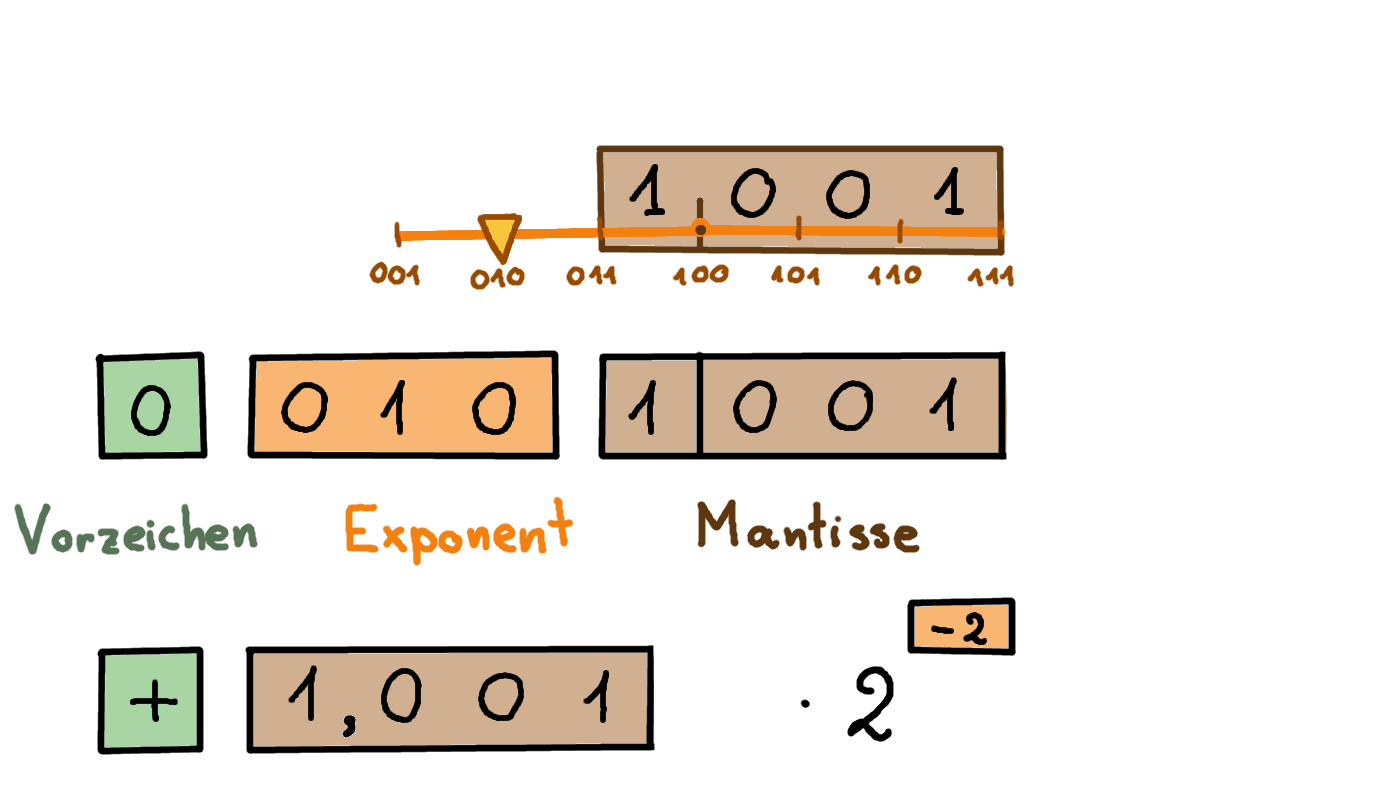
\includegraphics[width=0.8\linewidth]{Pictures/Einleitung_from_Kasten_Loesung.png} 
Den Dezimalwert berechenen wir, indem wir \((-1)^0 \cdot 1.001 \cdot 2^{-2} = 0.01001\) nach Dezimal konvertieren. In diesem Fall erhalten wir \(1/4 + 1/32 = 9/32\).
\end{figure}

\subsection{Fliesskommazahlen}

\paragraph{Aufgabe \ref{kleinsteZahl-5-3}}
Wir konstruieren die kleinste positive Zahl im Fliesskommazahlensystem mit Mantissenlänge \(5\) und Exponenten von \(-3\) bis \(3\).

Als erstes platzieren wir den Kasten. Damit die Zahl möglichst klein wird, muss der Kasten nach rechts möglichst weit weg vom Komma stehen. Wir haben aber eine Einschränkung: Das Seil muss immer mit dem Komma verbunden bleiben.
\begin{figure}[H]
\centering
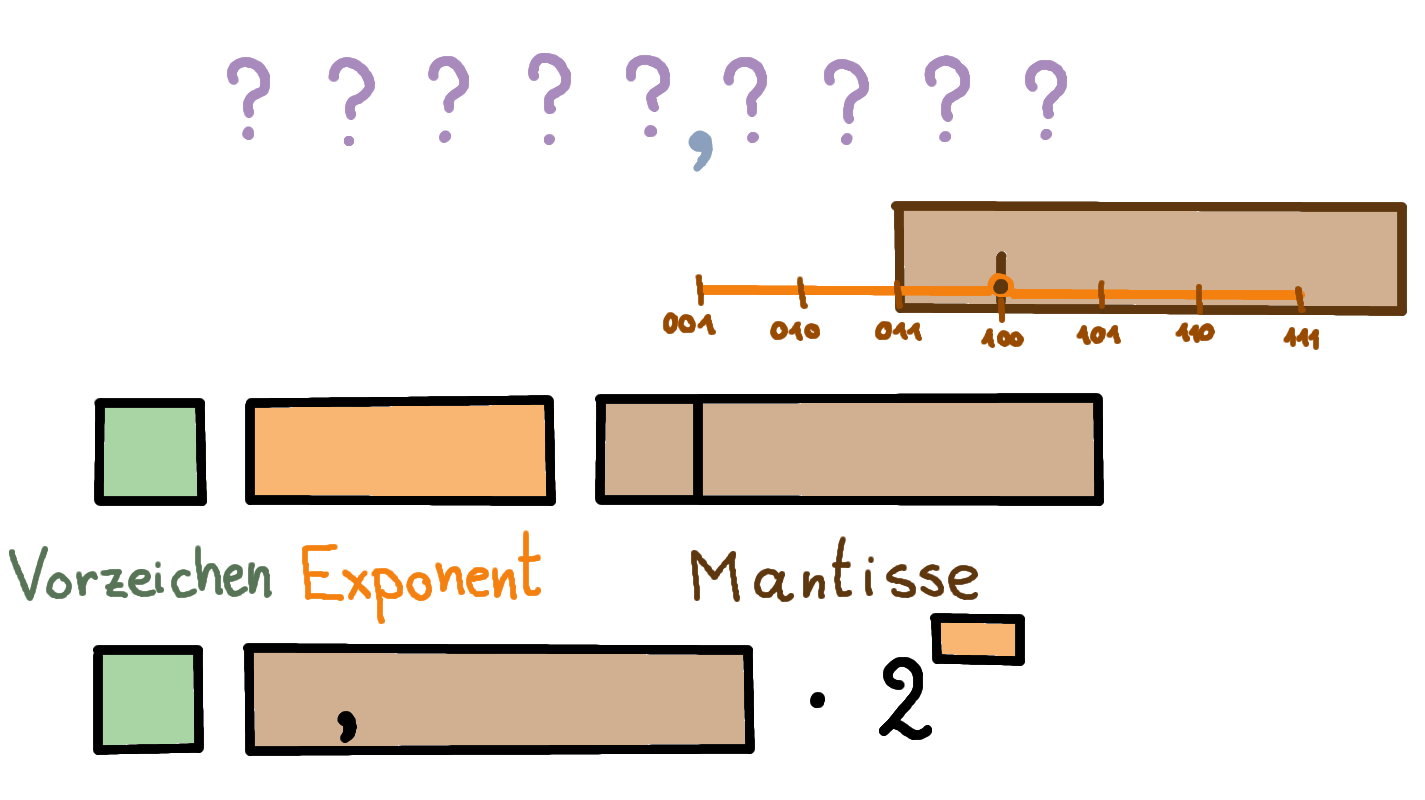
\includegraphics[width=0.85\linewidth]{Pictures/kleinsteZahl1.png}
\end{figure}
Der Exponent muss also möglichst klein sein.

Was ist mit der Mantisse? Sicher muss eine Eins an der ersten Stelle stehen.
\begin{figure}[H]
\centering
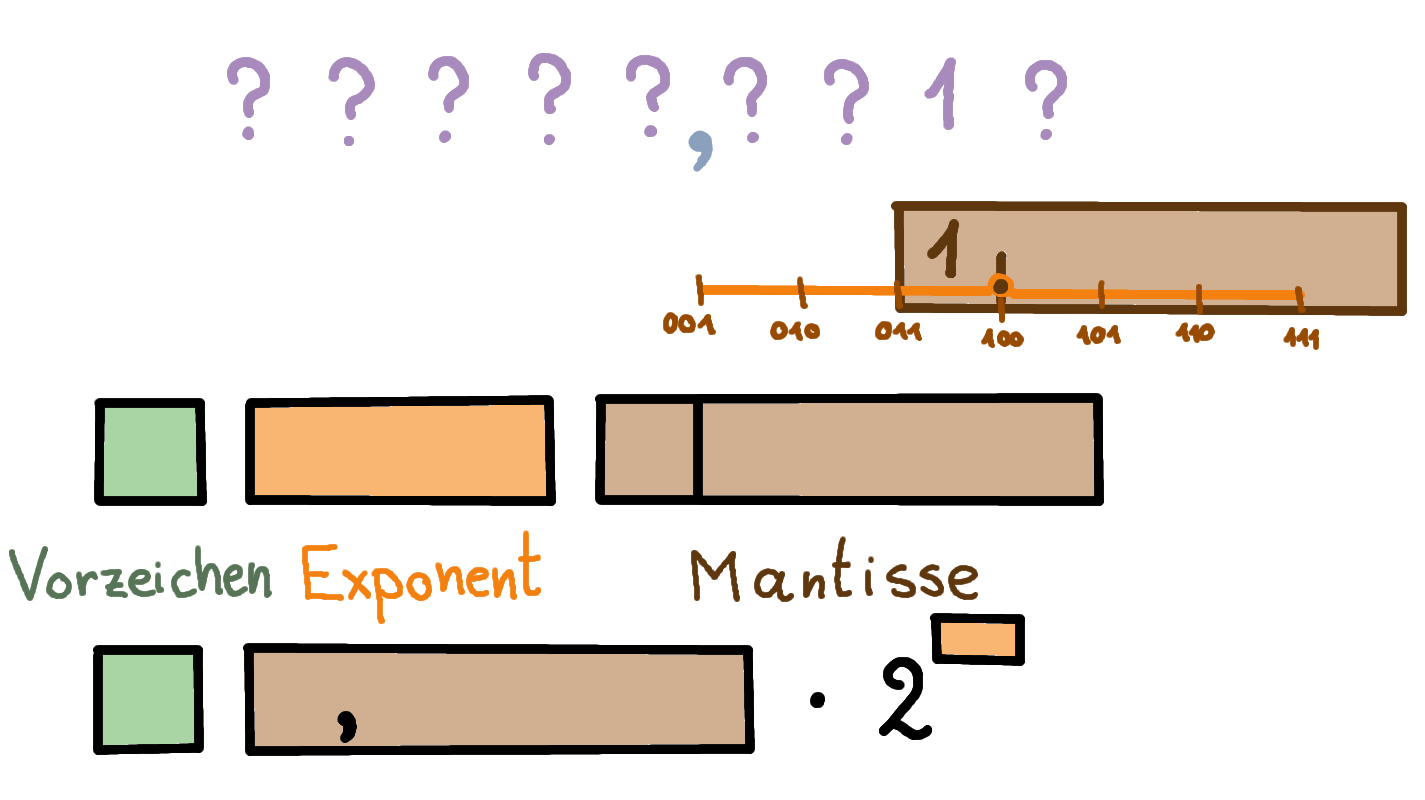
\includegraphics[width=0.85\linewidth]{Pictures/kleinsteZahl2.png}
\end{figure}

Damit die Mantisse möglichst klein wird, müssen wir so viele Stellen wie möglich auf Null setzen.
\begin{figure}[H]
\centering
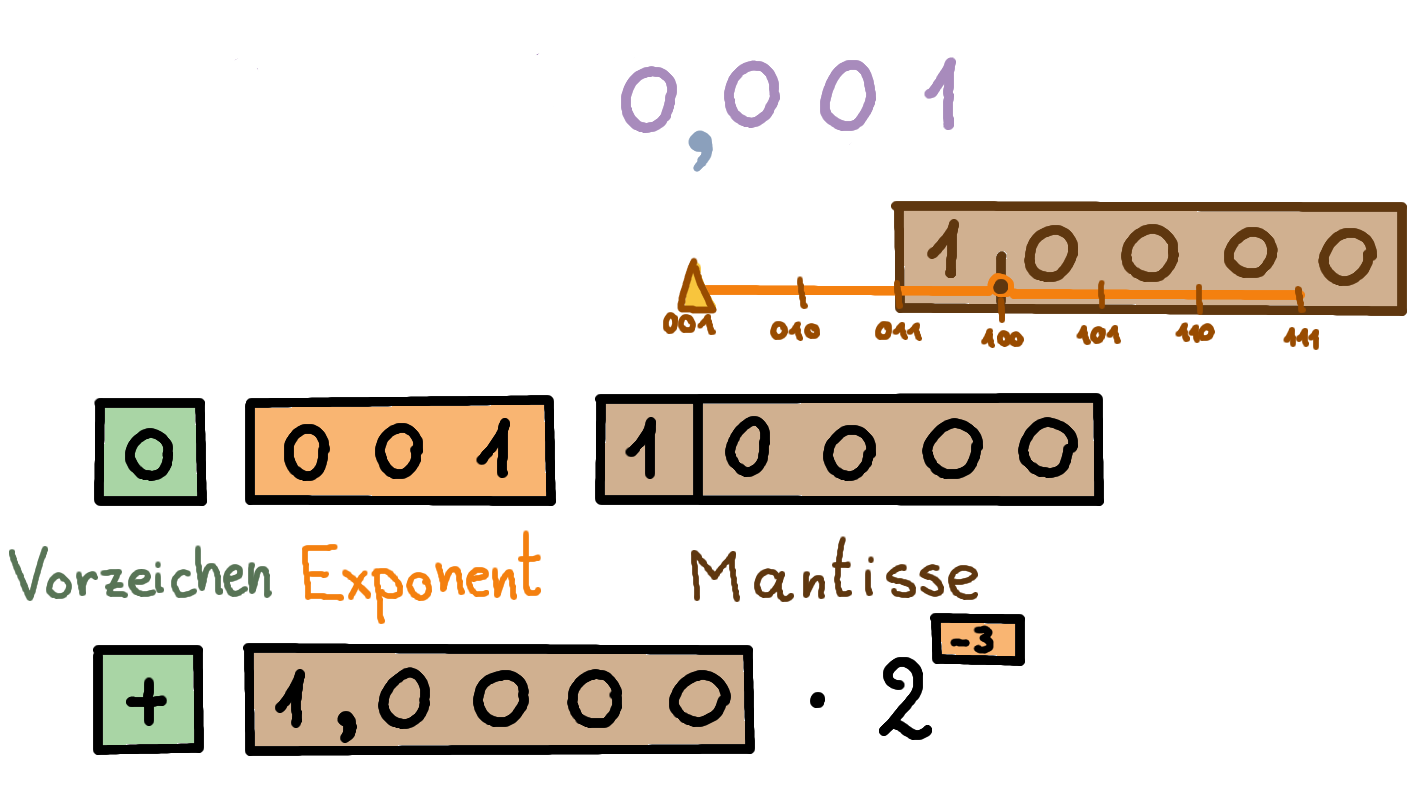
\includegraphics[width=0.85\linewidth]{Pictures/kleinsteZahl3.png}
\end{figure}

Die kleinste darstellbare Zahl in diesem Fliesskommazahlensystem ist also \(1/8\).

\paragraph{Aufgabe \ref{groesste-kleinste-4-3}}
Die grösste positive darstellbare Zahl in einem Fliesskommazahlensystem mit Mantissenlänge \(4\) und Exponent zwischen \(-3\) und \(3\) ist \(15\). Das ist nicht viel kleiner als \(15.5\), die grösste positive darstellbare Zahl in einem Fliesskommazahlensystem mit einem Bit mehr für die Mantisse.
\begin{figure}[H]
\centering
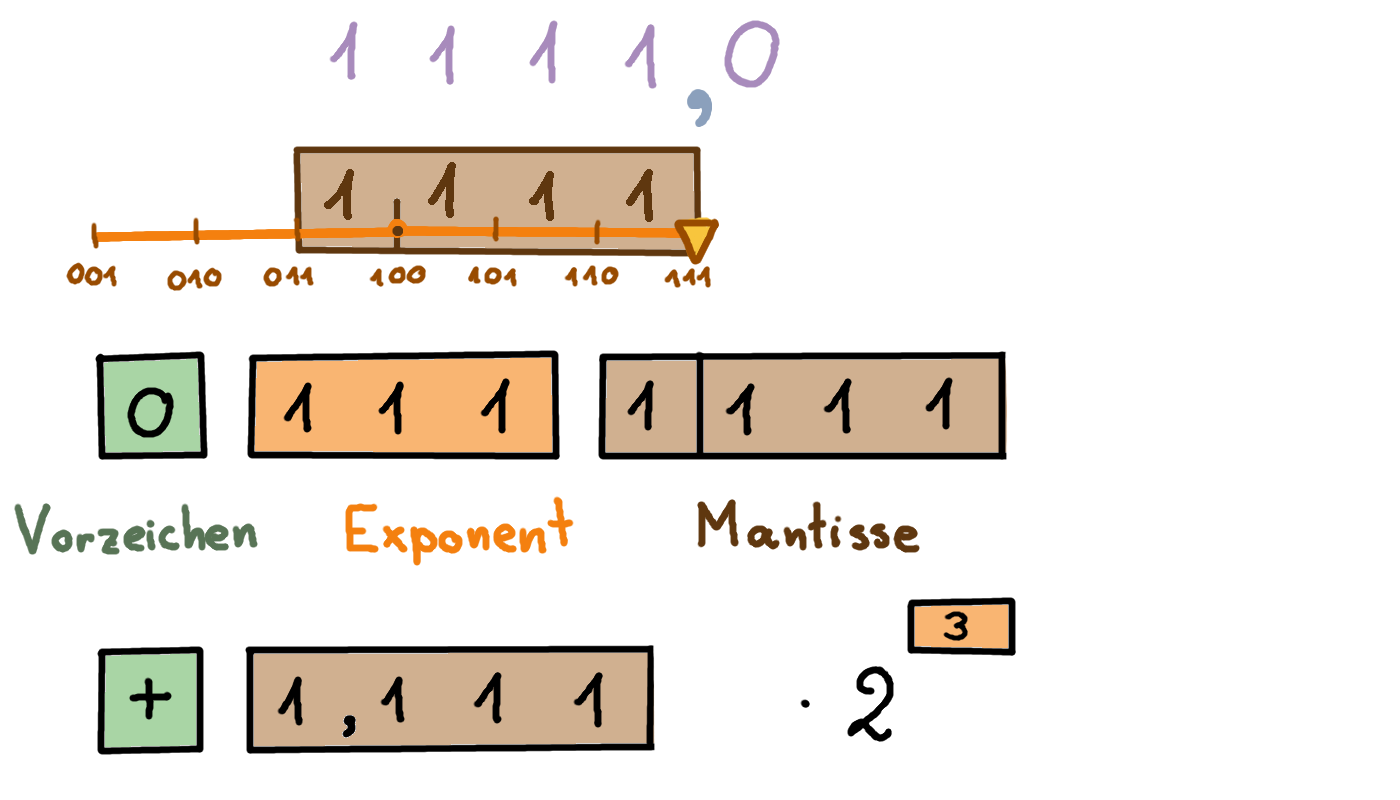
\includegraphics[width=0.85\linewidth]{Pictures/groessteZahl-4-3.png}
\end{figure}

Die kleinste positive darstellbare Zahl in einem Fliesskommazahlensystem mit Mantissenlänge \(4\) und Exponent zwischen \(-3\) und \(3\) ist auch \(1/8\), genau wie die kleinste positive darstellbare Zahl in einem Fliesskommazahlensystem mit einem Bit mehr für die Mantisse.
\begin{figure}[H]
\centering
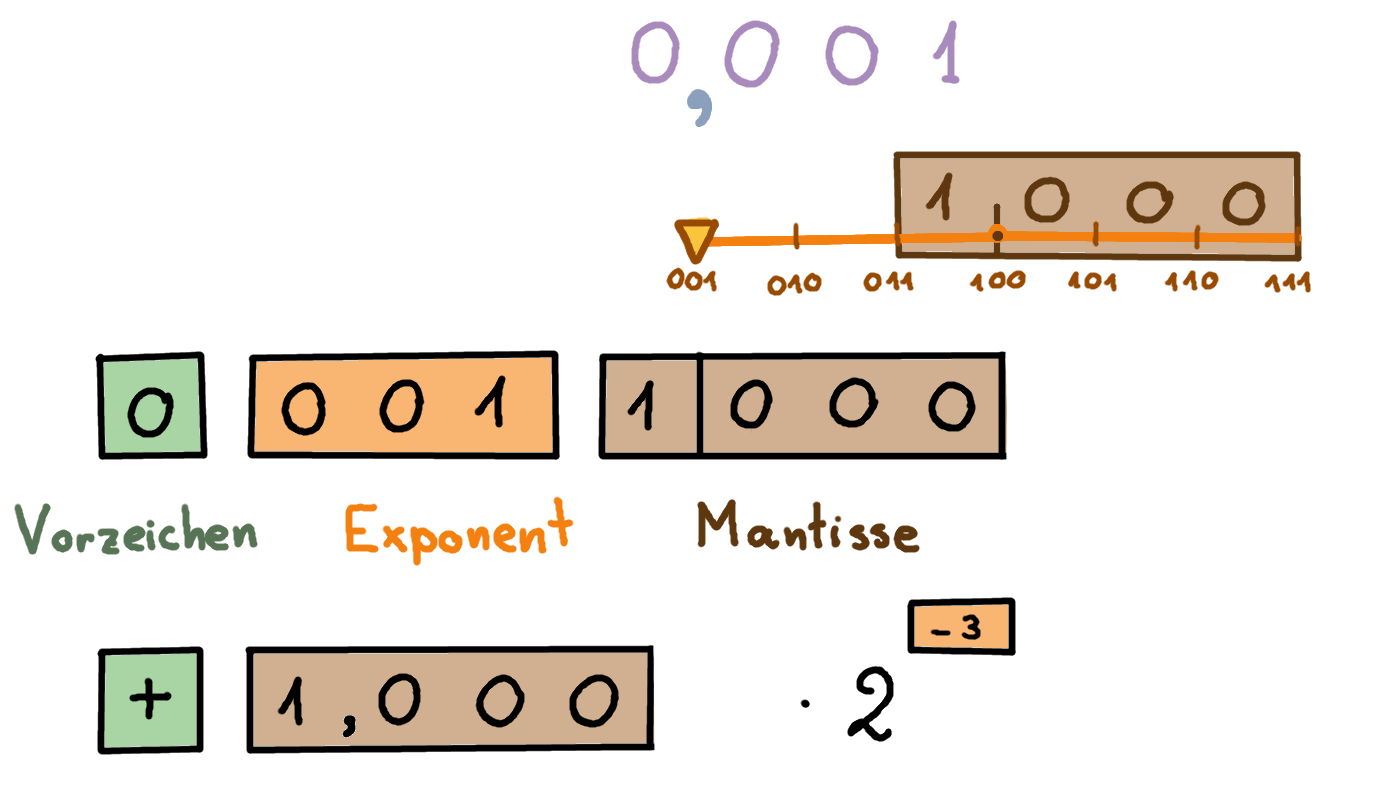
\includegraphics[width=0.85\linewidth]{Pictures/kleinsteZahl-4-3.png}
\end{figure}

Wie wir sehen, die Länge der Mantisse scheint wenig Einfluss auf die grösste und kleinste positive darstellbare Zahlen zu haben.

\paragraph{Aufgabe \ref{groesste-kleinste-5-2}}
\begin{enumerate}[(a)]
\item Der Exponent liegt zwischen \(-1\) und \(1\) und die mögliche Kodierungen sind \texttt{01, 10, 11}.
\item Die Erwartung ist, dass die grösste positive darstellbare Zahl deutlich kleiner wird, weil das Seil viel kürzer ist, und wir den Kasten nicht mehr so weit nach links ziehen können, wie im Fliesskommazahlensystem mit \(3\) Bits für den Exponenten. Analog, die kleinste positive darstellbare Zahl wird deutlich grösser.
\item Die grösste positive darstellbare Zahl in diesem System ist \(3+7/8 = 31/8\). Wie erwartet, das ist viel grösser als in einem Fliesskommazahlensystem mit einem Bit mehr für den Exponenten.
\begin{figure}[H]
\centering
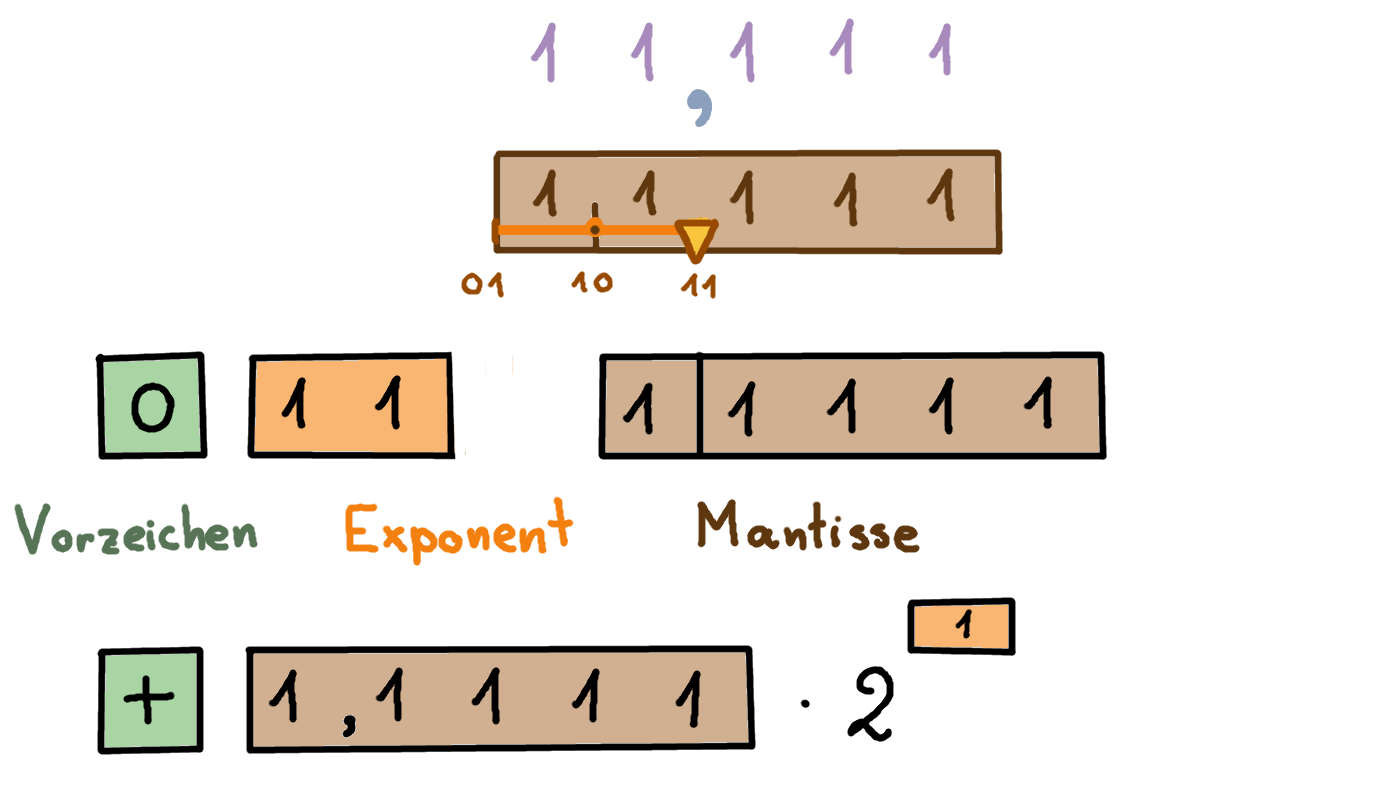
\includegraphics[width=0.85\linewidth]{Pictures/groessteZahl-5-2.png}
\end{figure}

Die kleinste positive darstellbare Zahl in diesem System ist \(0.5\). Das ist viel grösser als in einem Fliesskommazahlensystem mit einem Bit mehr für den Exponenten.
\begin{figure}[H]
\centering
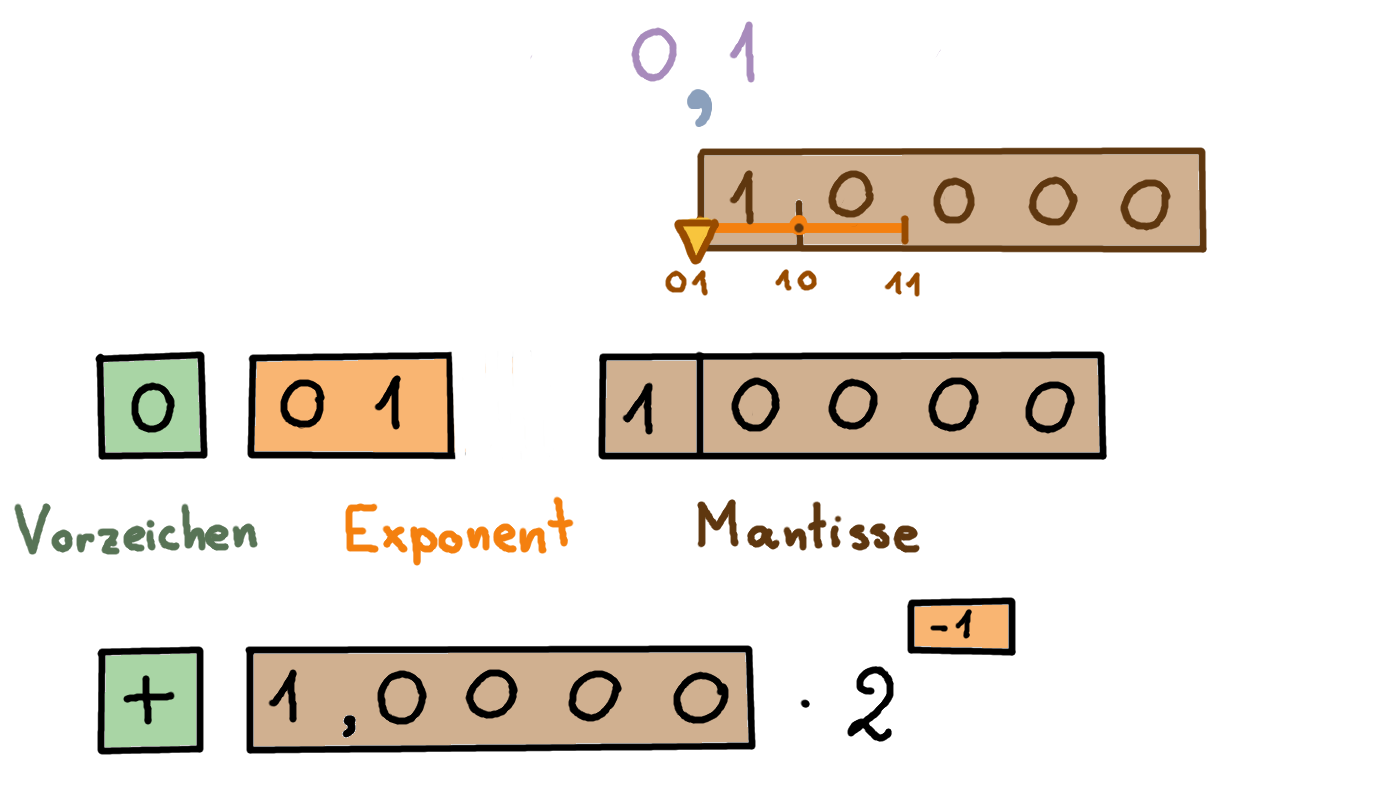
\includegraphics[width=0.85\linewidth]{Pictures/kleinsteZahl-5-2.png}
\end{figure}

\end{enumerate}


\paragraph{Aufgabe \ref{groesste-kleinste-allgemein}}

Im Allgemeinen für einen Fliesskommazahlensystem mit Mantissenlänge \(m\) und Exponenten zwischen \(e_{min}\) und \(e_{max}\) findet man die grösste und kleinste positive Zahlen wie folgt.

Für die grösste positive Zahl wählt man den grösstmöglichen Exponenten \(e_{max}\) und die grösstmögliche Mantisse \(1.111 \ldots 111\). In der Exponentialschreibweise ist die grösste Zahl also 
\[1.1111111 \ldots 111 \cdot 2^{e_{max}}\]
und hat das Bitmuster \texttt{0 1111...111 (1)111111...111}.

Für die kleinste positive Zahl wählt man den kleinsten möglichen Exponenten \(e_{min}\) und die kleinste mögliche Mantisse. Beachte, dass die Mantisse immer mit einer Eins starten muss. Die kleinste mögliche Mantisse ist deswegen \(1.0000 \ldots 000\). In der Exonentialschreibweise ist die kleinste Zahl also
\[1.0000000 \ldots 000 \cdot 2^{e_{min}}\]
und hat das Bitmuster \texttt{0 0000...001 (1)00000000...000}.
%--------------------------------

\paragraph{Aufgabe \ref{nachbarn-vorherige}}
Die nächstkleinste, oder vorherige, darstellbare Zahl finden wir, indem wir die Mantisse kleiner zu machen versuchen. Da die Mantisse von \(1\) die kleinste mögliche Mantisse ist, müssen wir den Exponenten um Eins zurücksetzen und die grösstmögliche Mantisse wählen.

\begin{figure}[H]
\centering
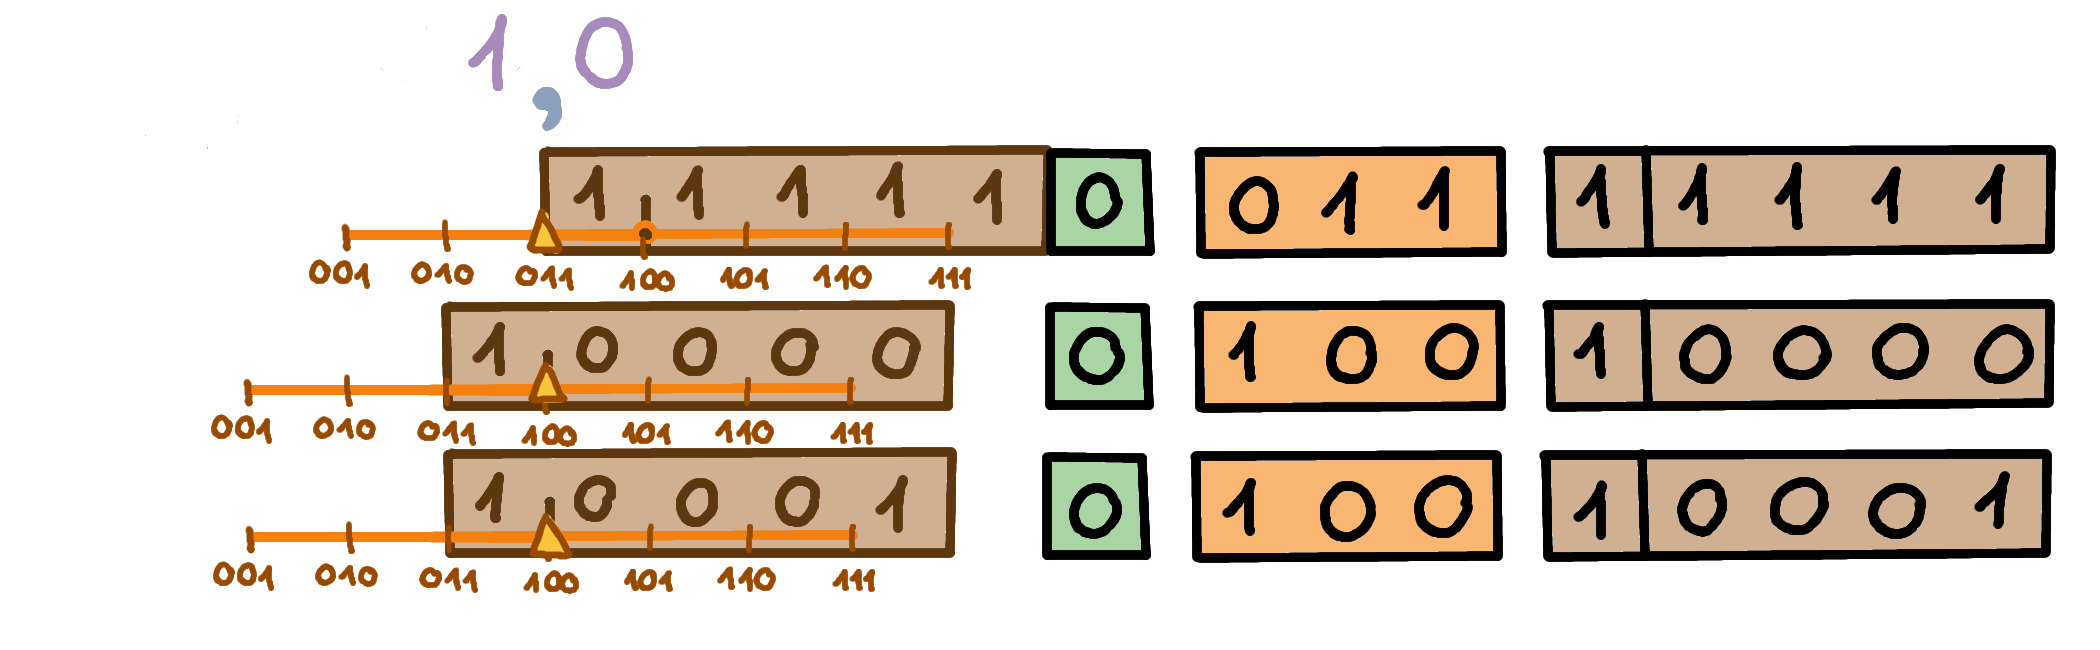
\includegraphics[width=\linewidth]{Pictures/Nachbarn1_P.png} 
\end{figure}
Die vorherige Zahl ist also \(31/32\).

Beachte, dass der Abstand zur nächsten und vorherigen darstellbaren Zahlen in diesem Fall nicht symmetrisch ist: die nächste Zahl ist \(1/16\) entfernt, während die vorherige nur \(1/32\).

\paragraph{Aufgabe \ref{nachbarn}}

\begin{enumerate}[(a)]
\item Die Nachbarn von \(2\) sind \(31/16\) und \(17/8\).
\begin{figure}[H]
\centering
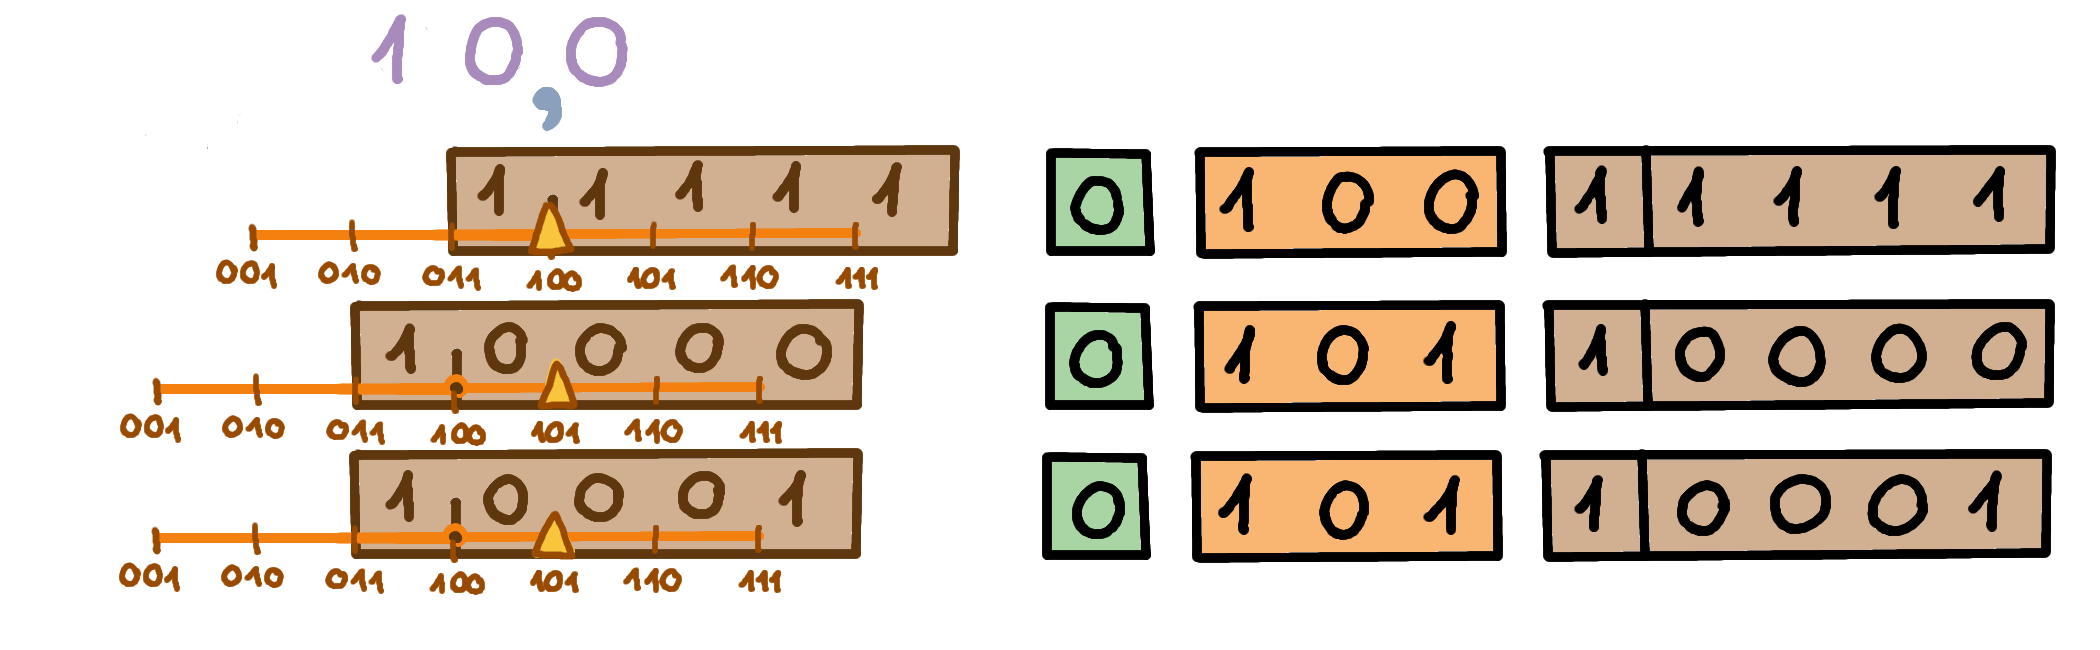
\includegraphics[width=\linewidth]{Pictures/Nachbarn2.png}
\end{figure}

\item Die Nachbarn von \(3\) sind \(23/8\) und \(25/8\).
\begin{figure}[H]
\centering
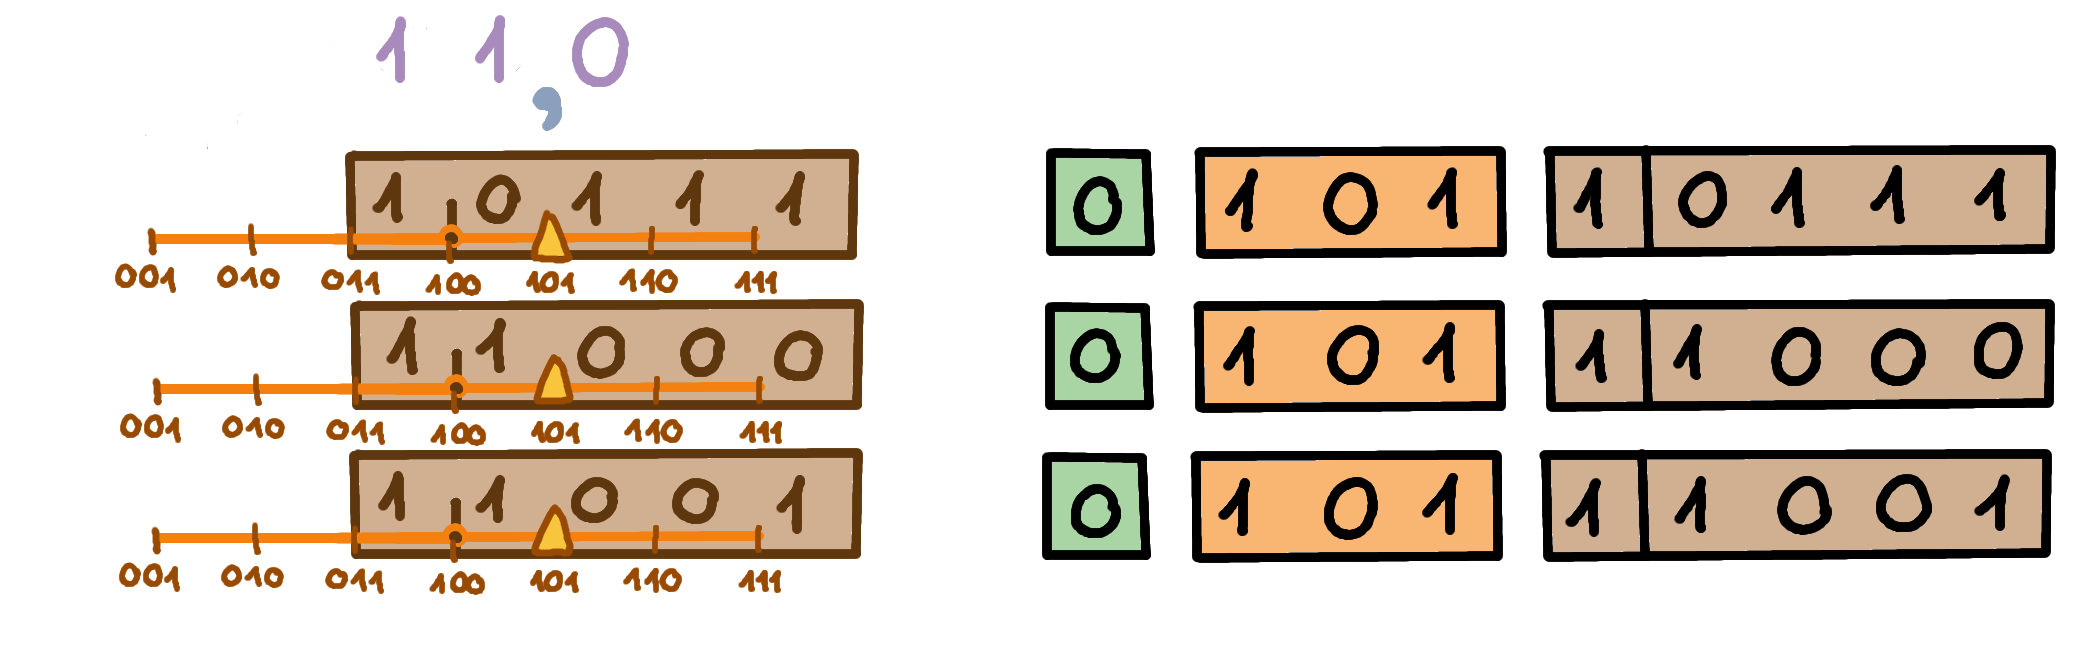
\includegraphics[width=\linewidth]{Pictures/Nachbarn3.png}
\end{figure}

\item Die Nachbarn von \(4\) sind \(31/8\) und \(17/4\).
\begin{figure}[H]
\centering
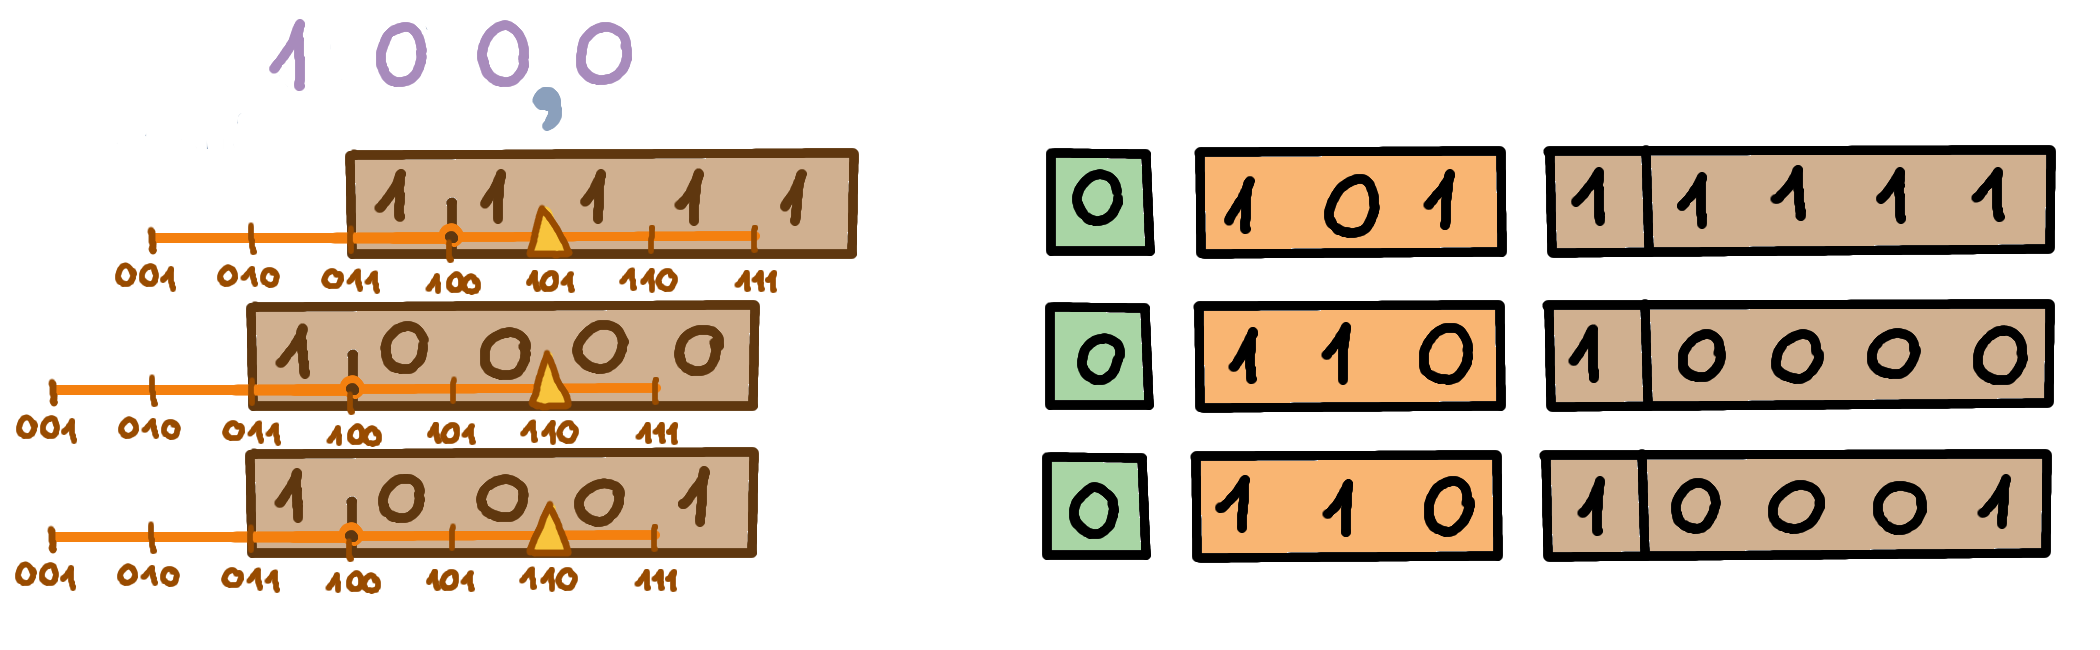
\includegraphics[width=\linewidth]{Pictures/Nachbarn4.png}

Die positive darstellbare Zahlen sind auf dem Zahlenstrahl nicht gleichverteilt.
\end{figure}

\end{enumerate}

\paragraph{Aufgabe \ref{nachbarn-laenge}}
\begin{enumerate}[(a)]
\item Im Fliesskommazahlensystem mit Mantissenlänge \(4\) und Exponent zwischen \(-3\) und \(3\) sind die Nachbarn von \(1\): \(15/16\) und \(9/8\).
\begin{figure}[H]
\centering
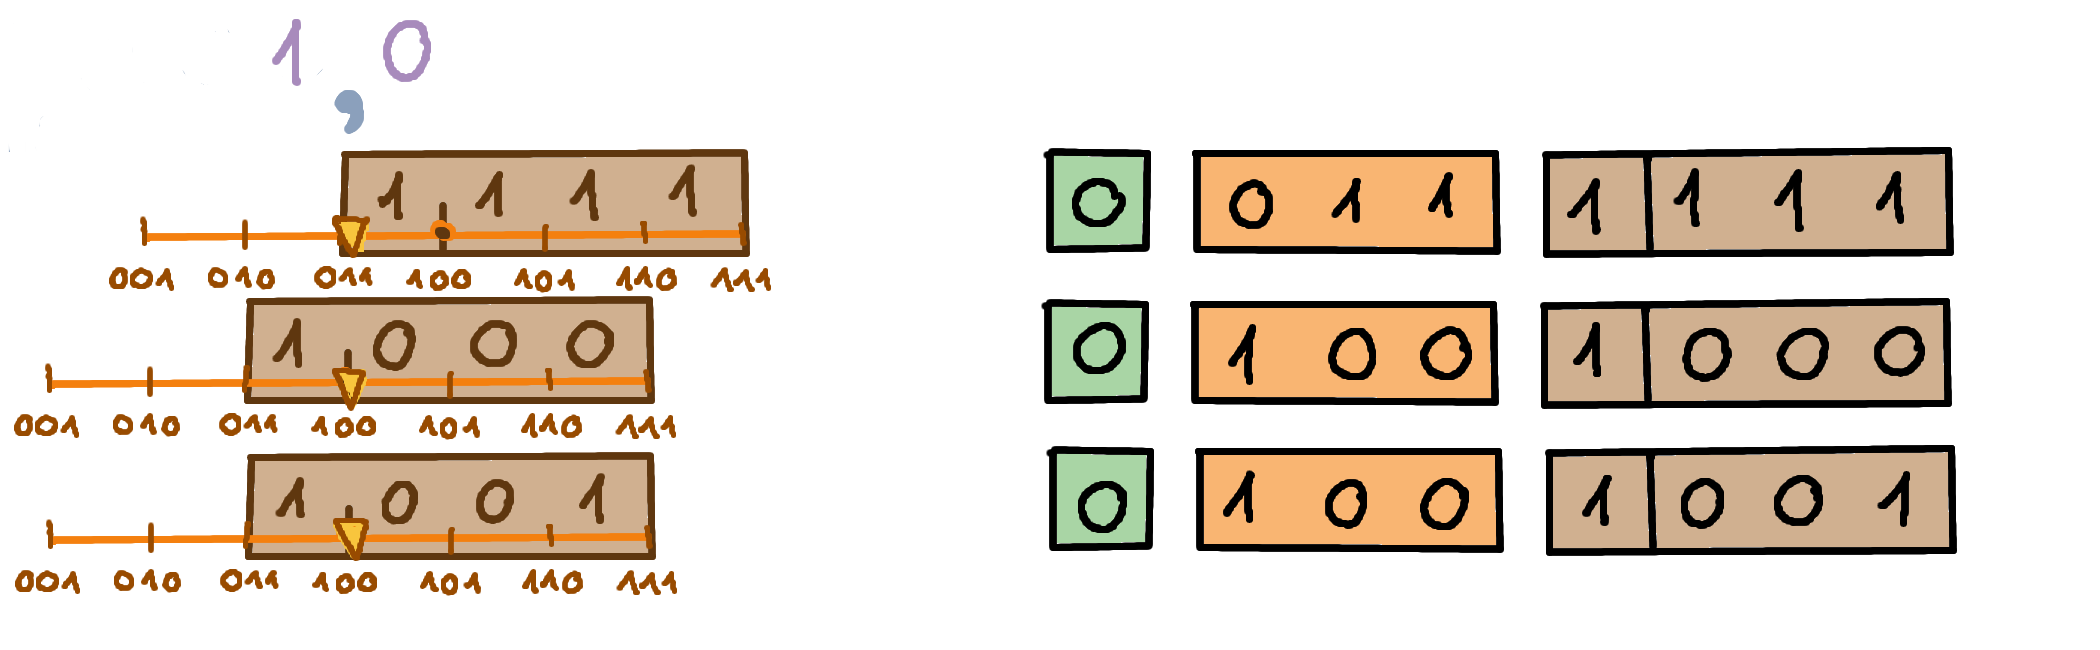
\includegraphics[width=\linewidth]{Pictures/Nachbarn1-4-3-Loesung.png}
\end{figure}

\item Im Fliesskommazahlensystem mit Mantissenlänge \(5\) und Exponent zwischen \(-1\) und \(1\) sind die Nachbarn von \(1\): \(31/32\) und \(17/16\).
\begin{figure}[H]
\centering
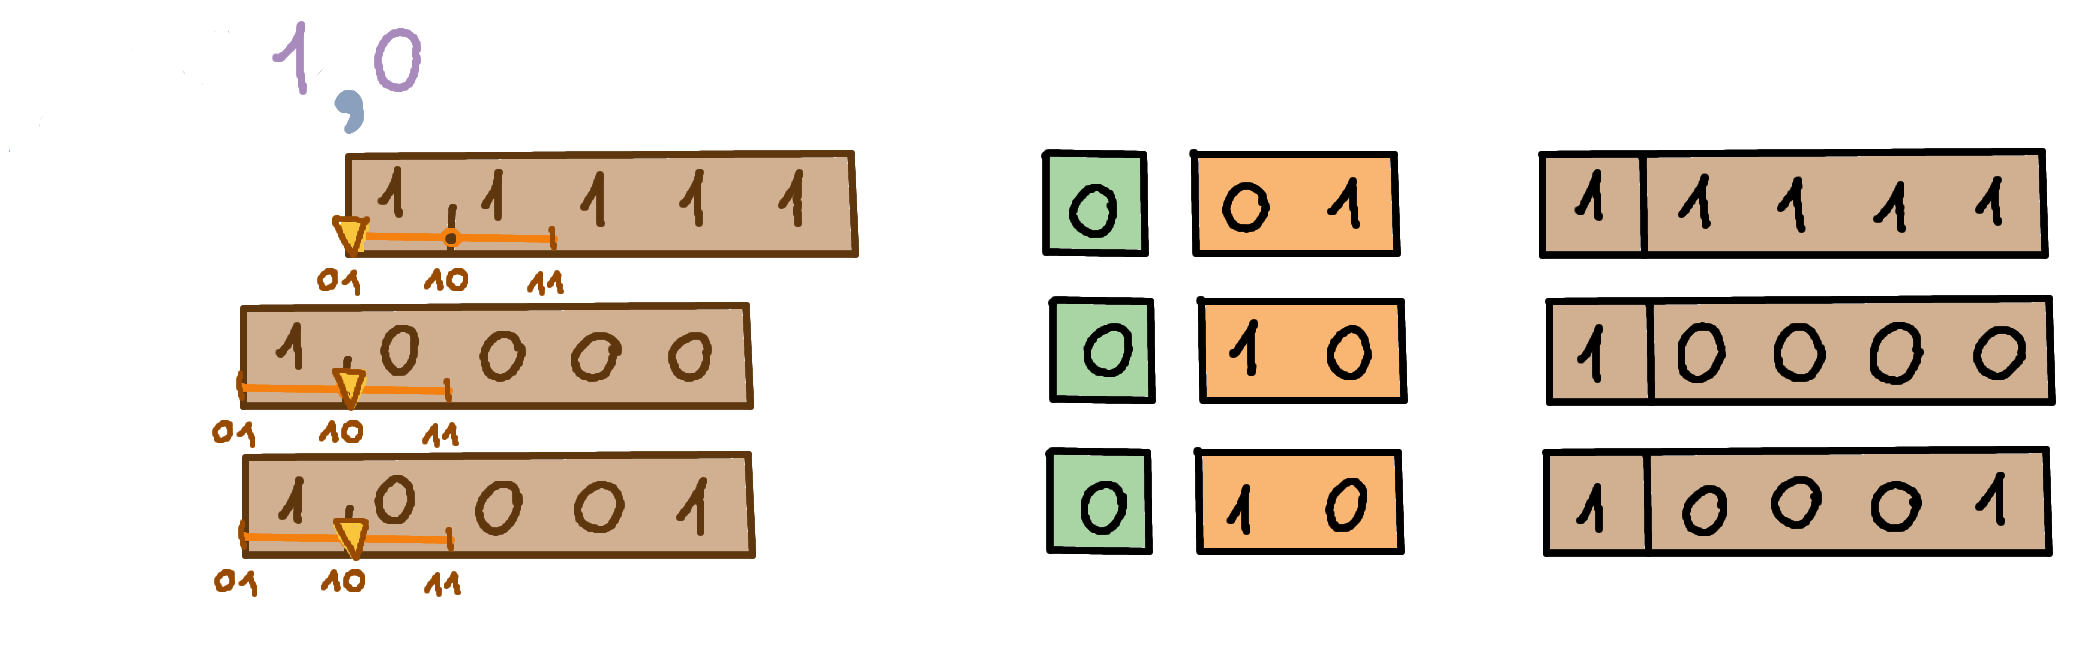
\includegraphics[width=\linewidth]{Pictures/Nachbarn1-5-2-Loesung.png}
\end{figure}

\item Die Länge der Mantisse beeinflusst den Abstand zwischen darstellbaren Zahlen stärker als die Länge der Exponentenkodierung. Wenn der Kasten grösser ist, gibt es mehr Platz für signifikante Stellen und Zahlen können genauer approximiert werden. Das führt dazu, dass der Abstand zwischen darstellbaren Zahlen kleiner wird.
\end{enumerate}

%--------------------------------

\paragraph{Aufgabe \ref{fliesskommazahlen_kontrollfragen}}
\begin{enumerate}[(a)]
\item Nein, es gibt unendlich viele reelle Zahlen und endlich viele Fliesskommazahlen.
\item Ja, die grösste Zahl ist \(1.1111 \ldots 111 \cdot 2^{e_{max}}\).
\item Ja, die kleinste Zahl ist \(1.0000 \ldots 000 \cdot 2^{e_{min}}\).
\item Die Länge der Exponentenkodierung beeinflusst den Bereich stärker als die Mantissenlänge. Wenn das Seil länger ist, kann man den Kasten weiter weg vom Komma platzieren und viel grössere oder kleinere Zahlen darstellen.
\item Zum Beispiel, die Zahl \(2.25\) lässt sich in diesem System nicht exakt darstellen. In der binären Exponentialschreibweise diese Zahl ist \(1.001 \cdot 2^{1}\). Um diese Zahl exakt zu speichern bräuchten wir \(4\) Bits für die Mantisse, wir haben aber nur \(3\).
\item Nein, die darstellbare Fliesskommazahlen sind nicht gleichverteilt. Die kleineren stehen dichter beieinander, weil bei kleineren Zahlen die letzte Stelle der Mantisse weniger Wert ist.
\item Die Mantissenlänge beeinflusst stärker den Abstand zwischen positiven darstellbaren Zahlen in einem Fliesskommazahlensystem. Wenn der Kasten mehr Plätze hat, kann man mehr Stellen speichern und somit Zahlen genauer darstellen.
\end{enumerate}

%--------------------------------

\subsection{Addition}
\paragraph{Aufgabe \ref{addition}}
\begin{enumerate}[(a)]
\item \(5/8 + 3/4 = 11/8\), in der Exponentialschreibweise \(1.0110 \cdot 2^{0}\)

Im ersten Schritt schreiben wir die Zahlen auf.
\begin{figure}[H]
\centering
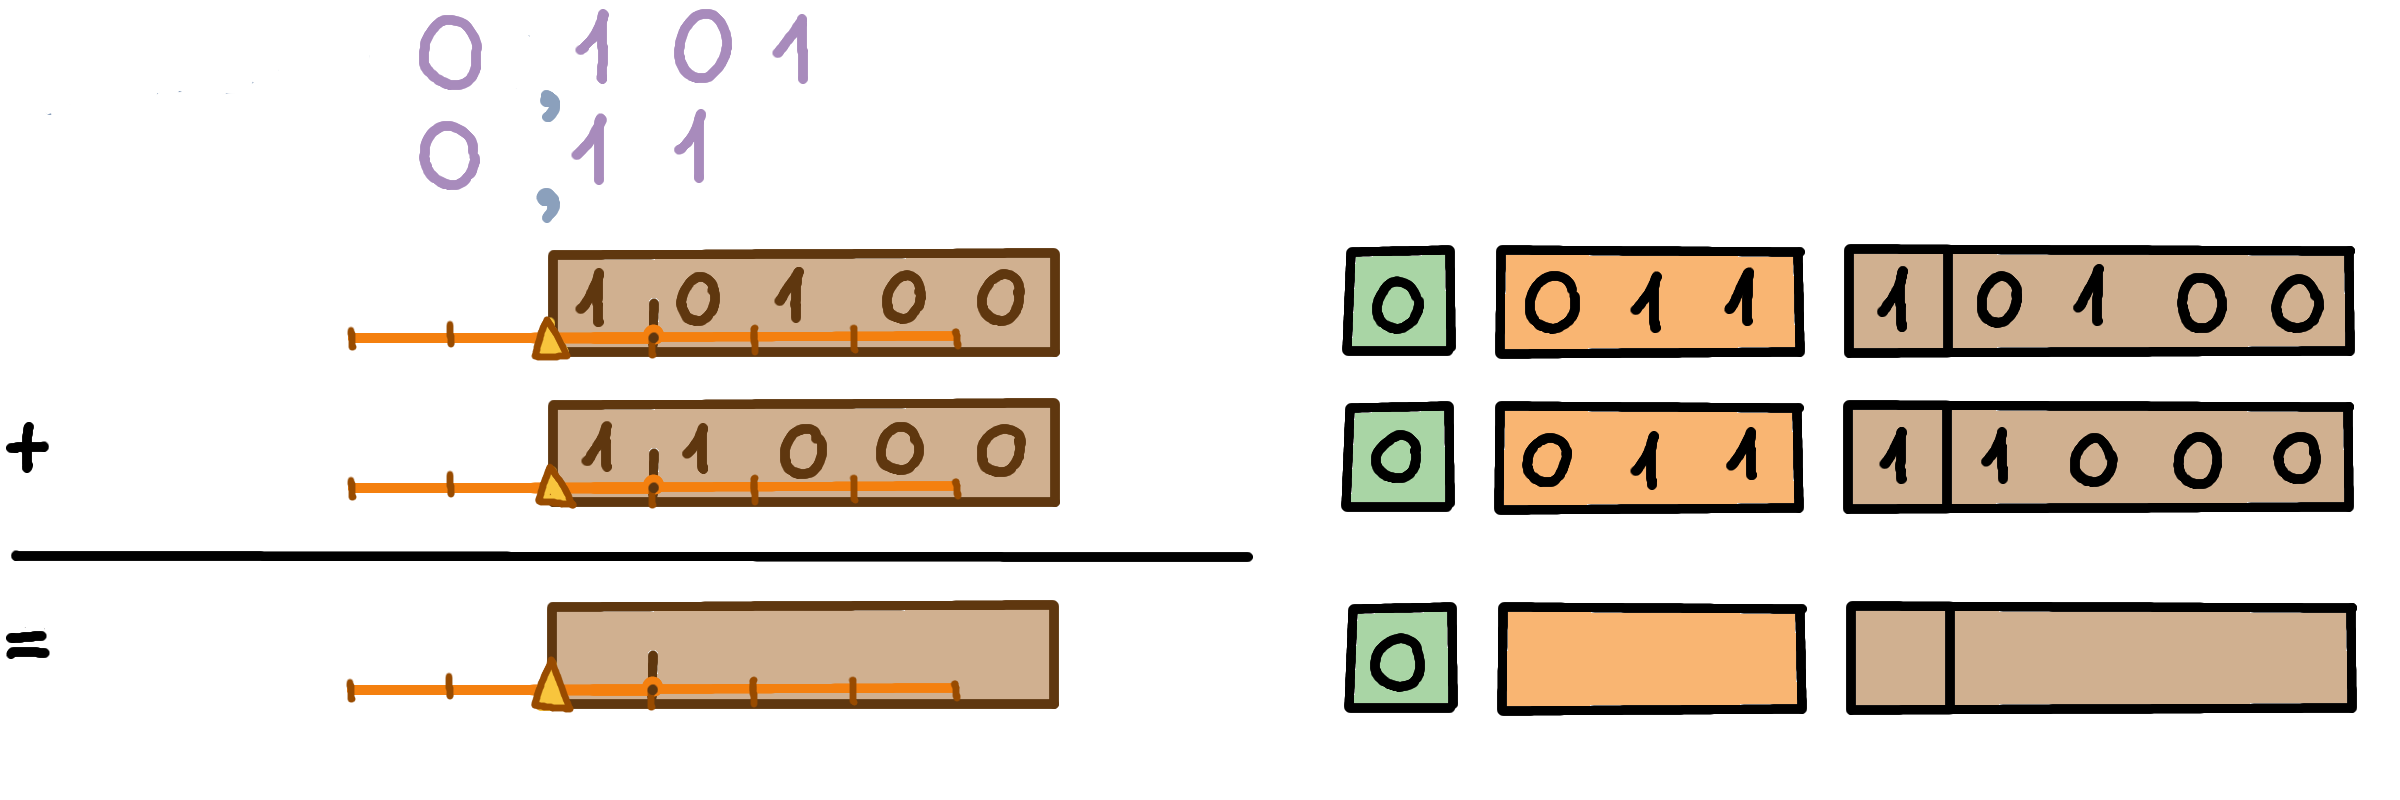
\includegraphics[width=\linewidth]{Pictures/Addition5-8and3-4_1.png}
\end{figure}
Da die zwei Kasten schon übereinander liegen, müssen wir sie nicht verschieben und können die Bits stellenweise zusammen addieren.
\begin{figure}[H]
\centering
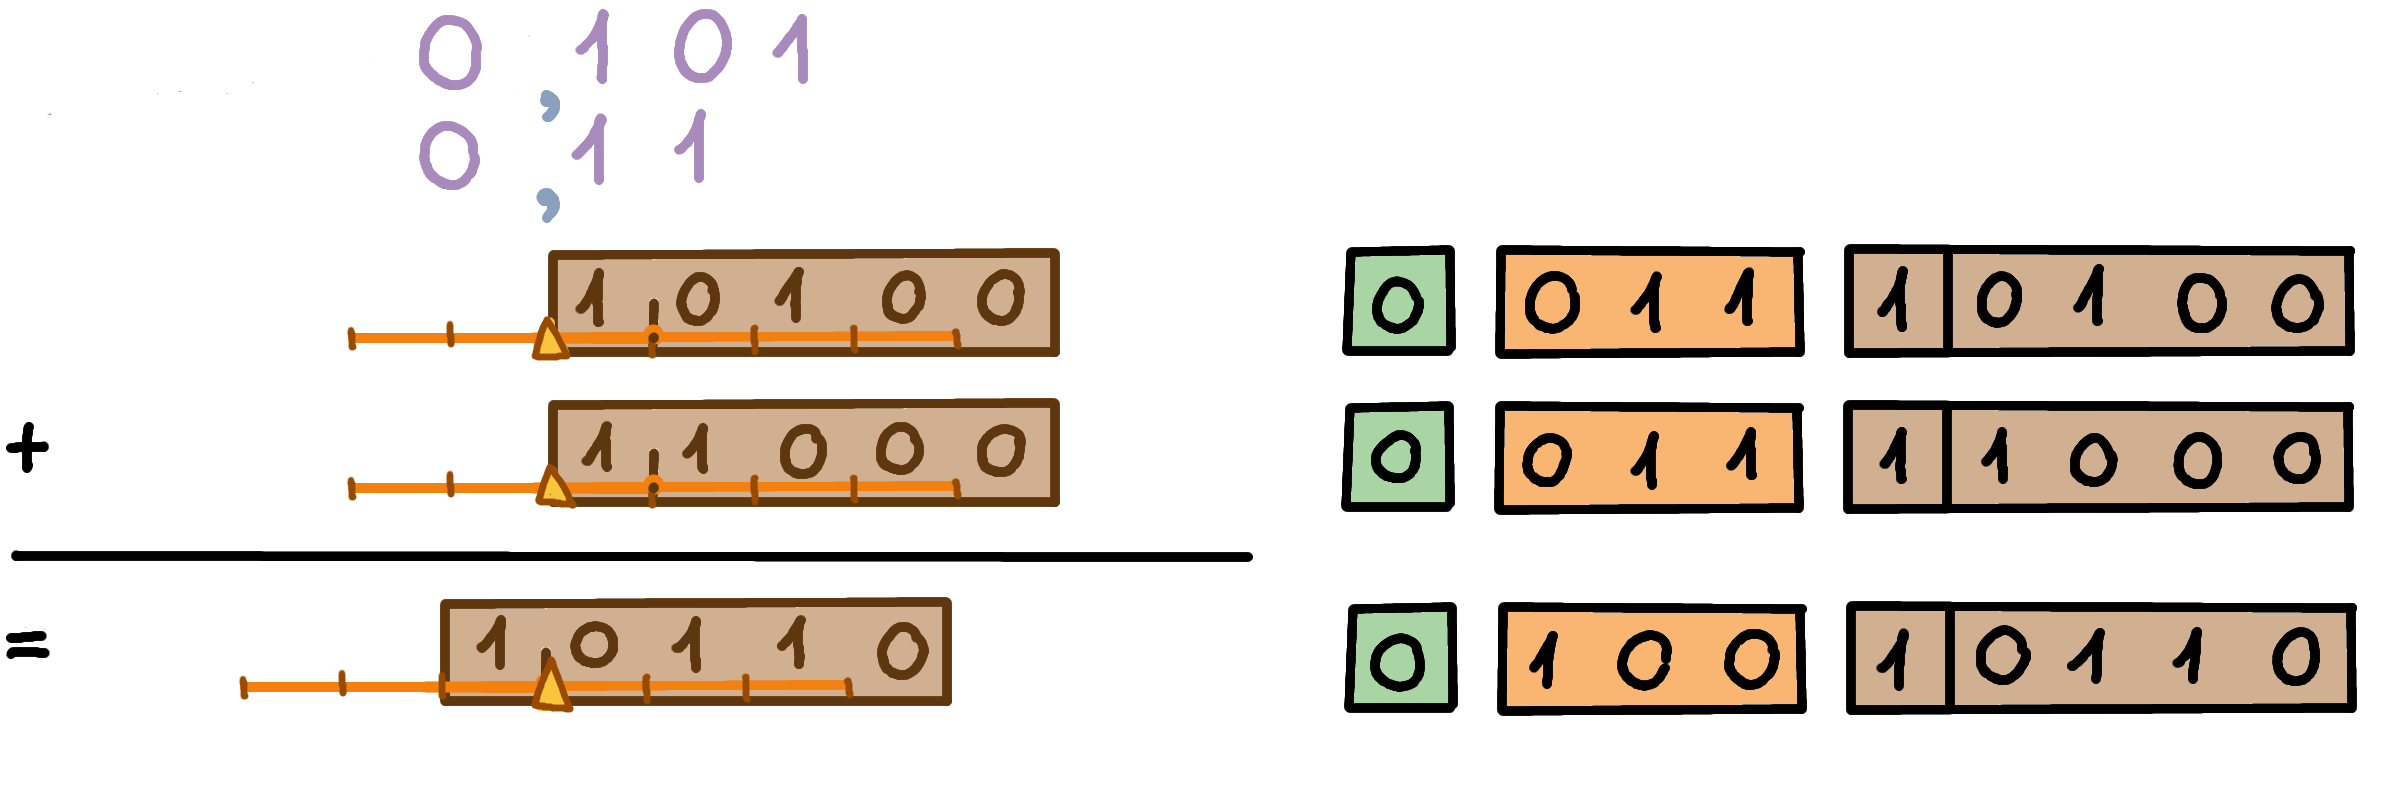
\includegraphics[width=\linewidth]{Pictures/Addition5-8and3-4_2.png}
\end{figure}
Der Kasten vom Ergebnis ist verschoben bezüglich den Kasten der Summanden.

\item \(10 + 2.25 = 12\), in der Exponentialschreibweise \(1.1000 \cdot 2^3\)

Im ersten Schritt schreiben wir die Zahlen auf.
\begin{figure}[H]
\centering
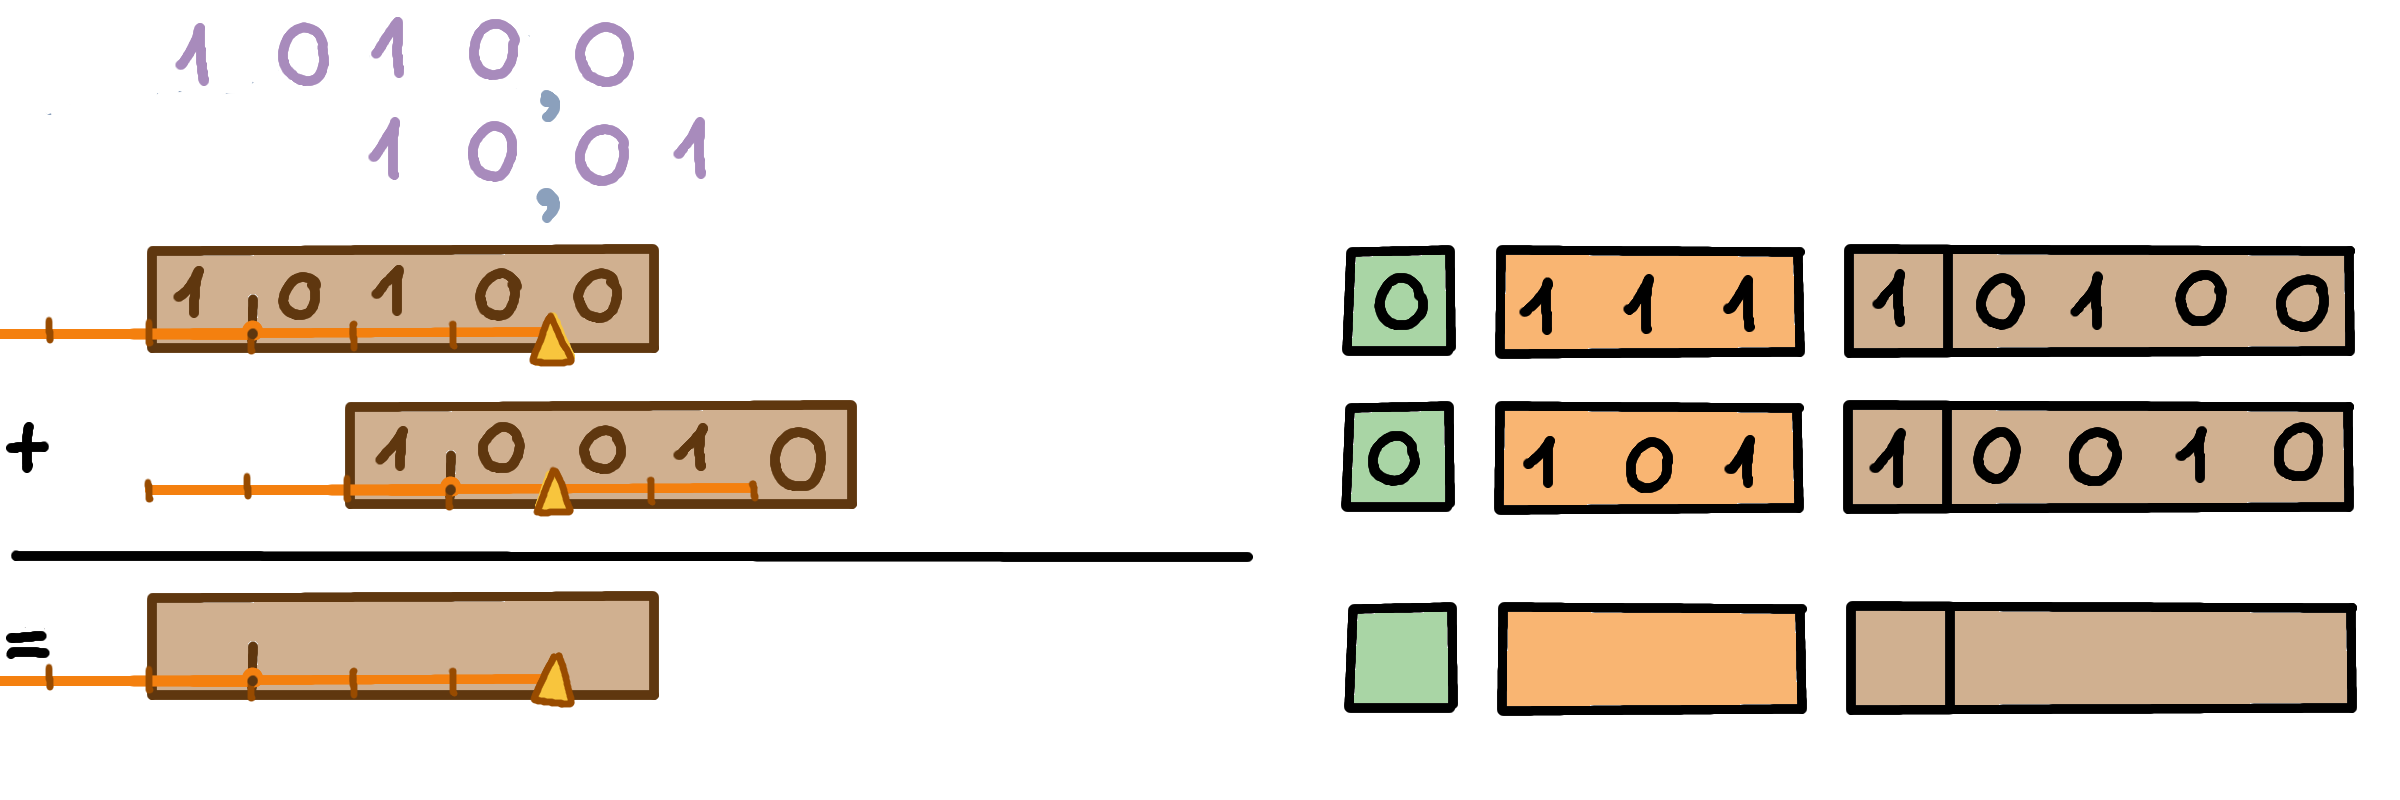
\includegraphics[width=\linewidth]{Pictures/Addition10and2-25_1.png}
\end{figure}

Im zweiten Schritt schiben wir den Kasten von der kleinsten Zahl unter den Kasten der grössten Zahl. Dabei gehen zwei Stellen verloren, eine davon ist eine Eins.
\begin{figure}[H]
\centering
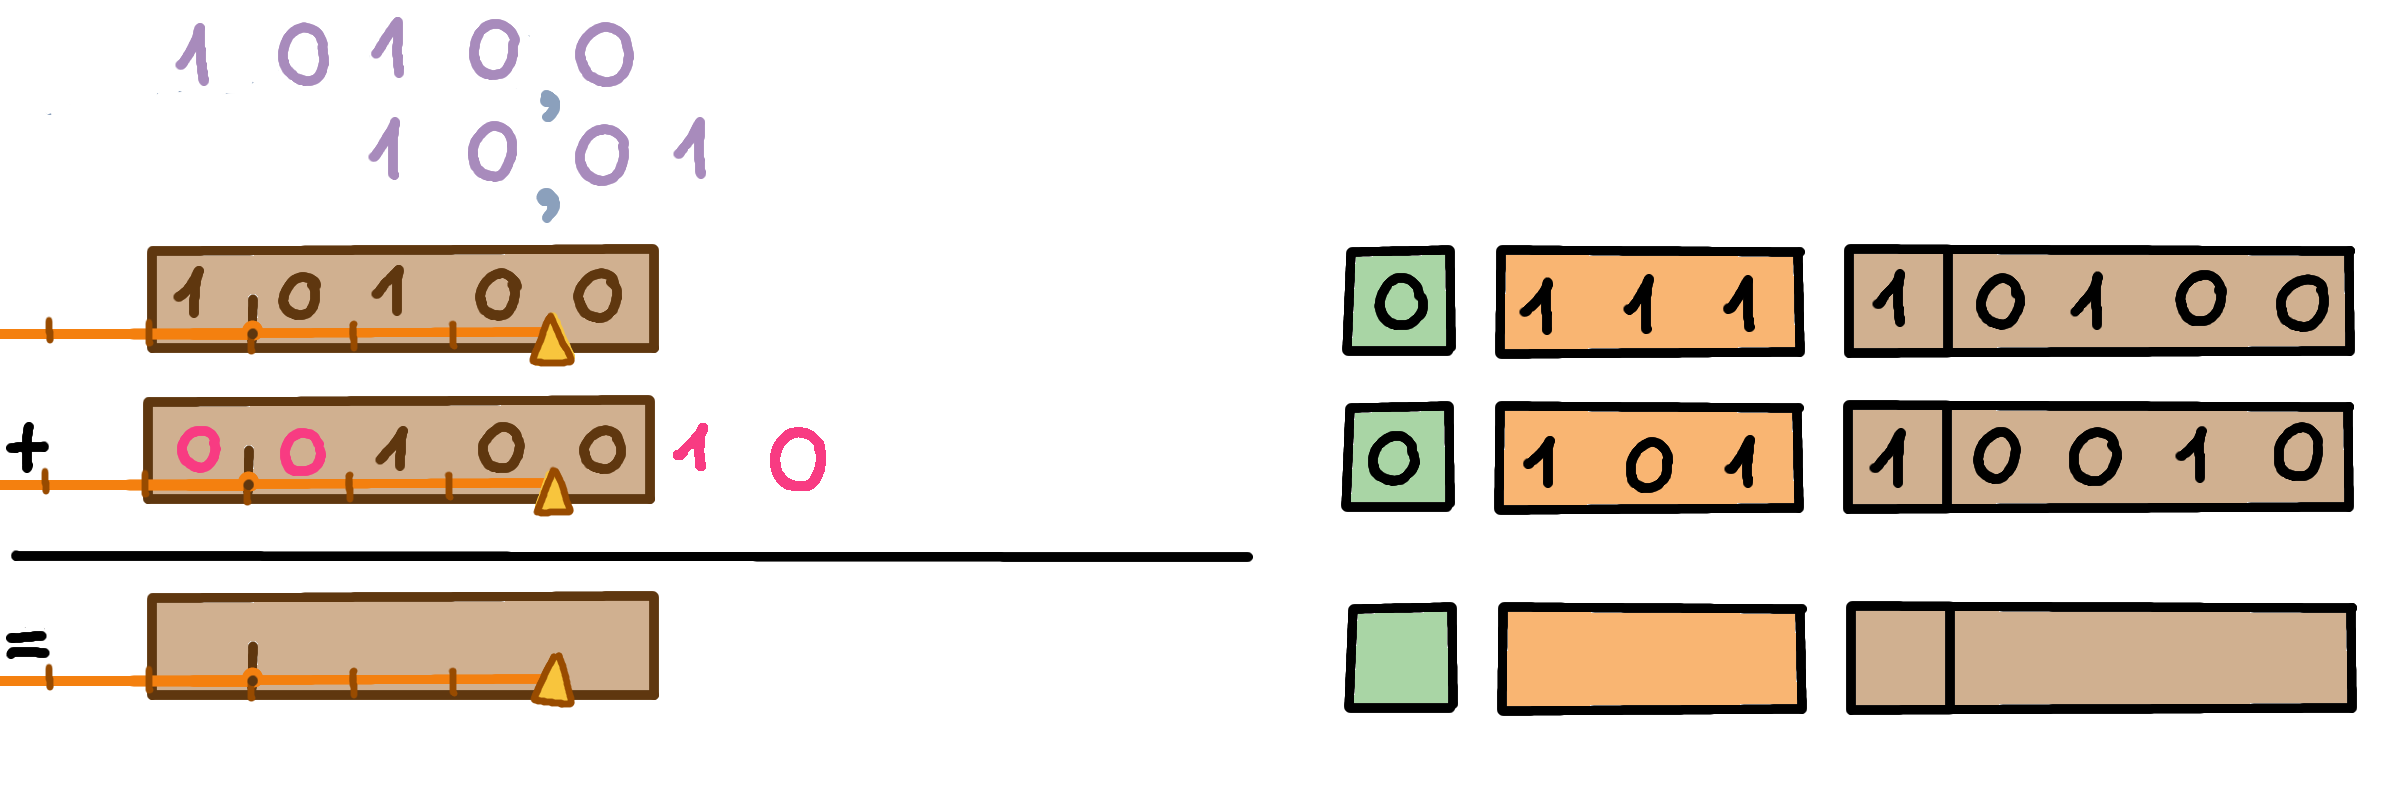
\includegraphics[width=\linewidth]{Pictures/Addition10and2-25_2.png}
\end{figure}

Nun können wir die Bits stellenweise zusammenrechnen.
\begin{figure}[H]
\centering
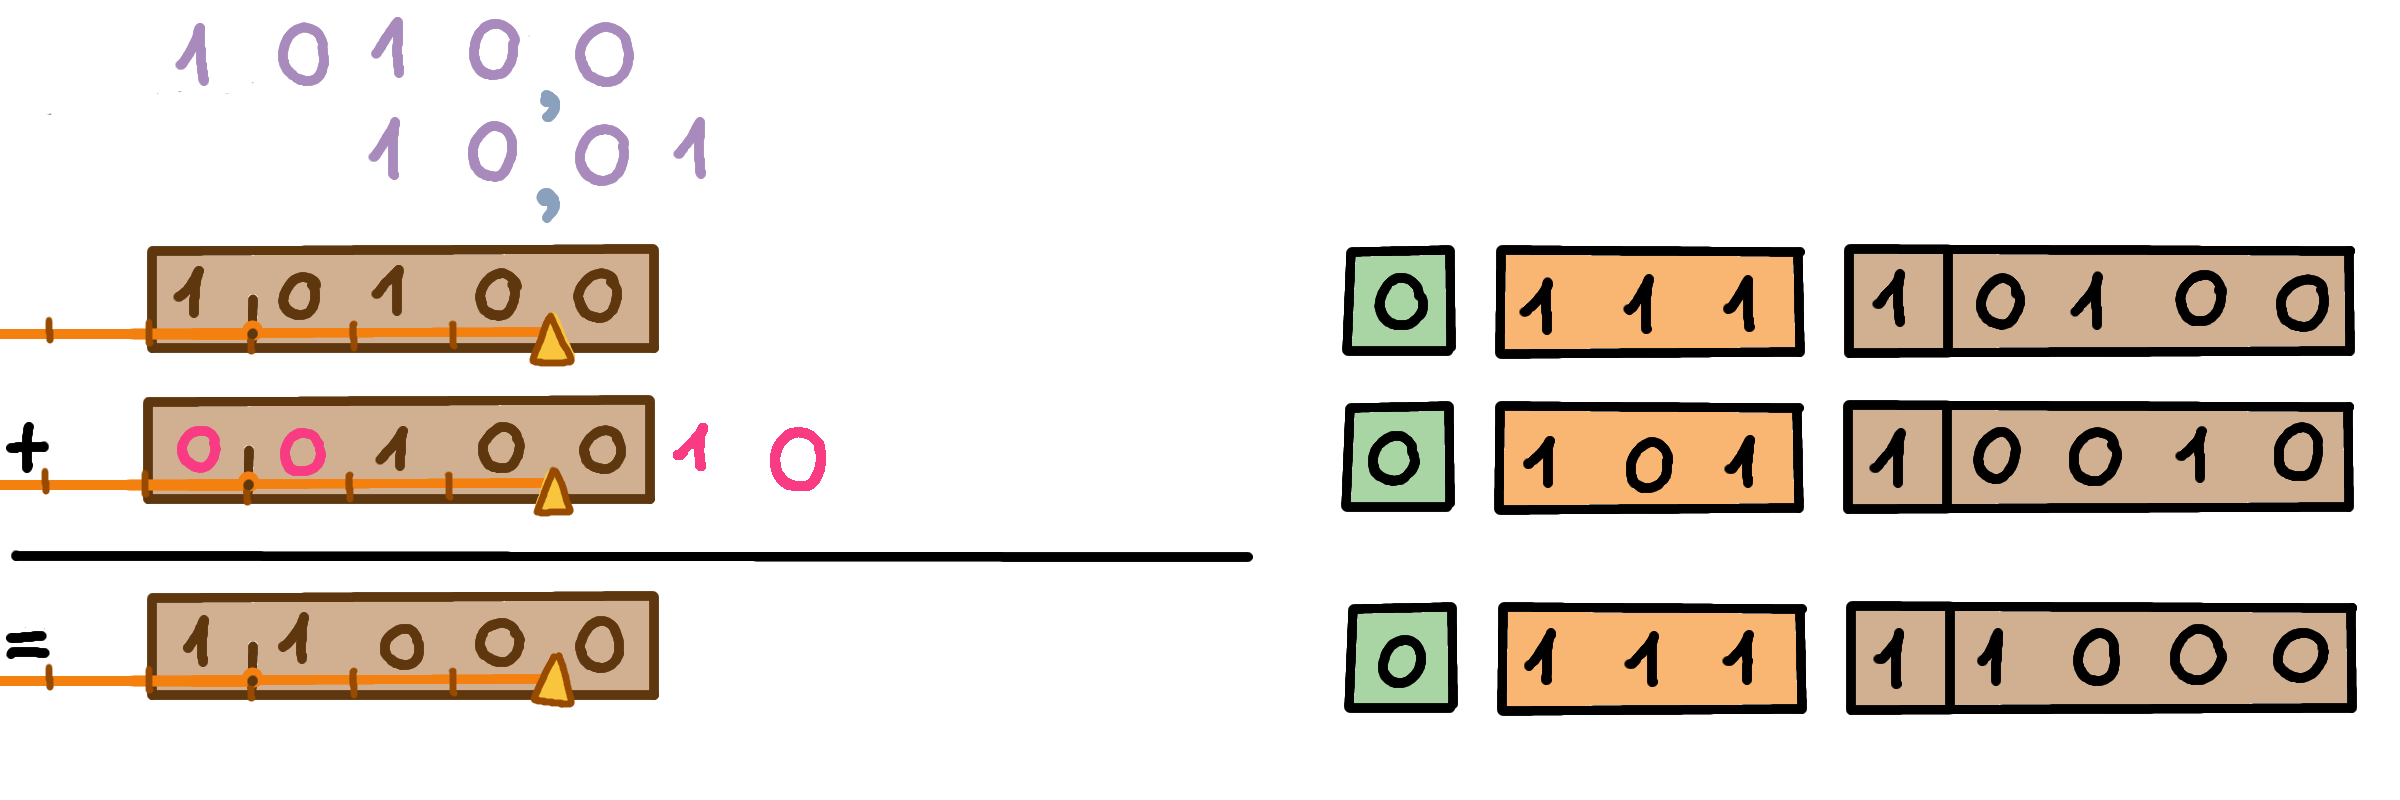
\includegraphics[width=\linewidth]{Pictures/Addition10and2-25_3.png}
\end{figure}

\item \(17/16 + 2 = 3\), in der Exponentialschreibweise \(1.1000 \cdot 2^1\).

Im ersten Schritt schreiben wir die Zahlen auf.
\begin{figure}[H]
\centering
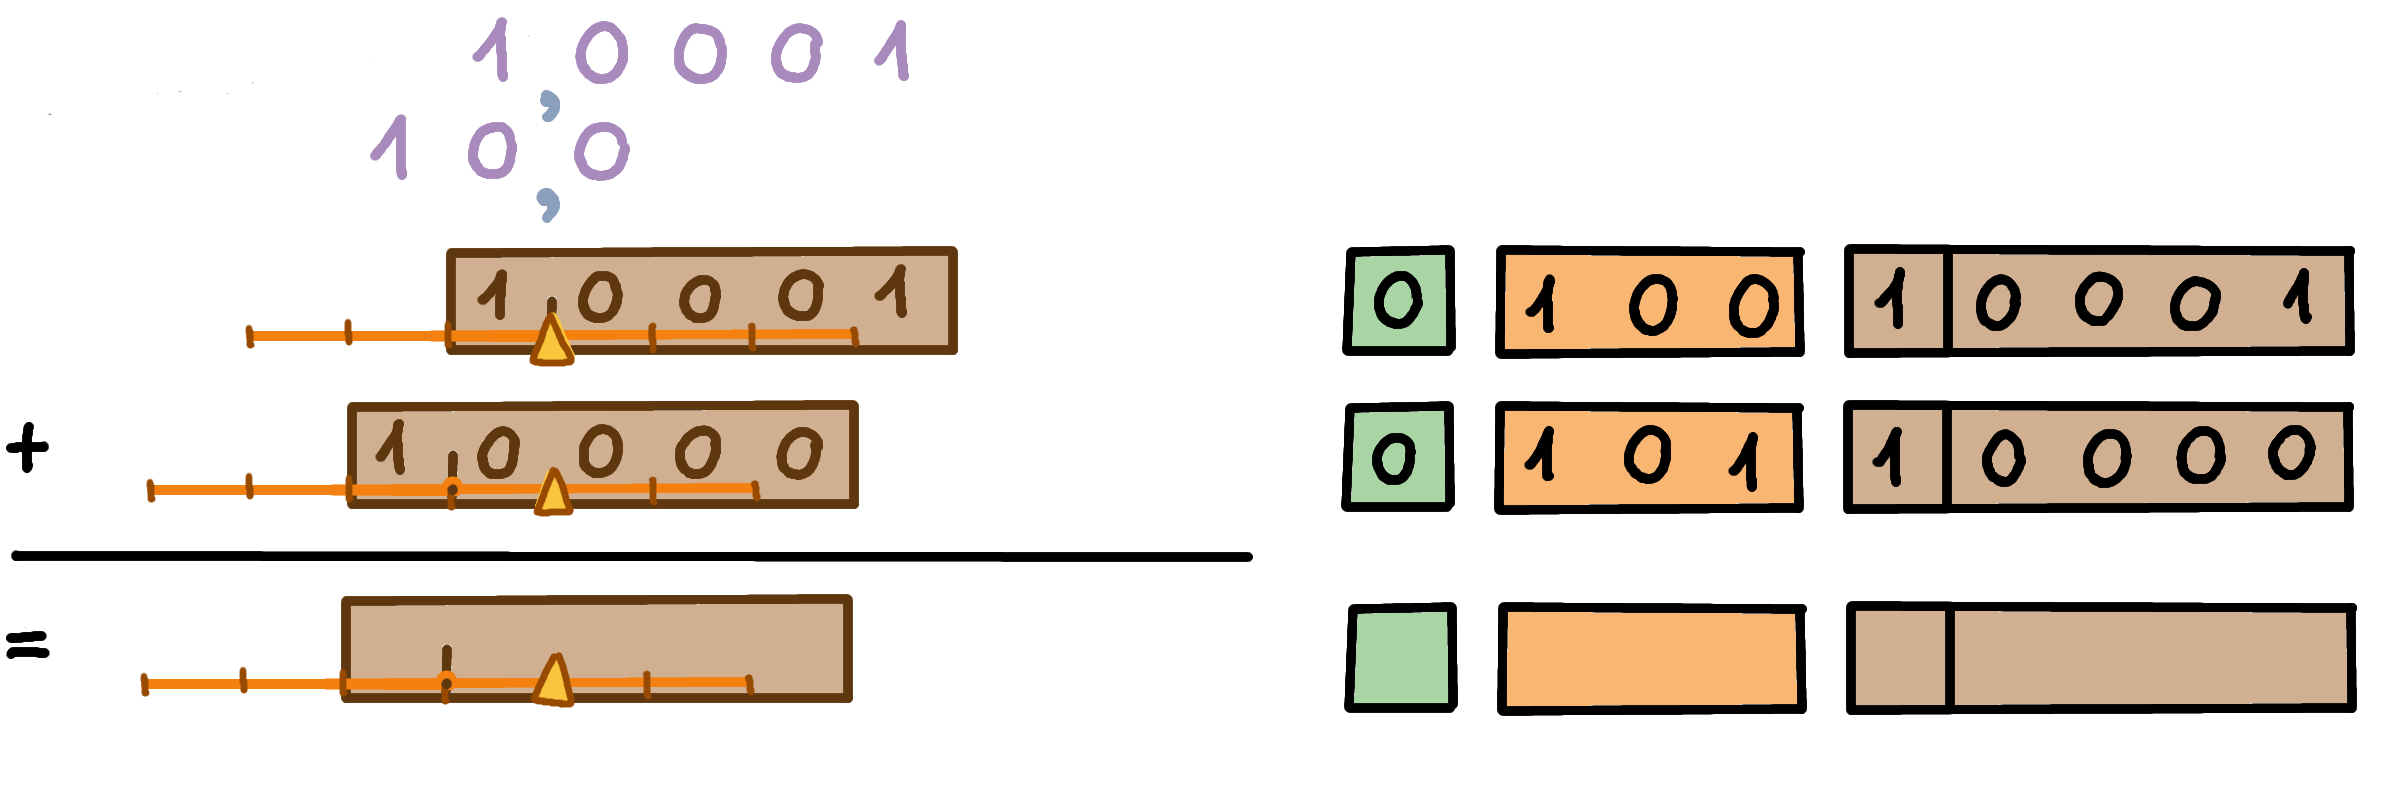
\includegraphics[width=\linewidth]{Pictures/Addition17-16and2_1.png}
\end{figure}

Im zweiten Schritt schiben wir den Kasten von der kleinsten Zahl unter den Kasten der grössten Zahl. Dabei geht eine Stelle verloren.
\begin{figure}[H]
\centering
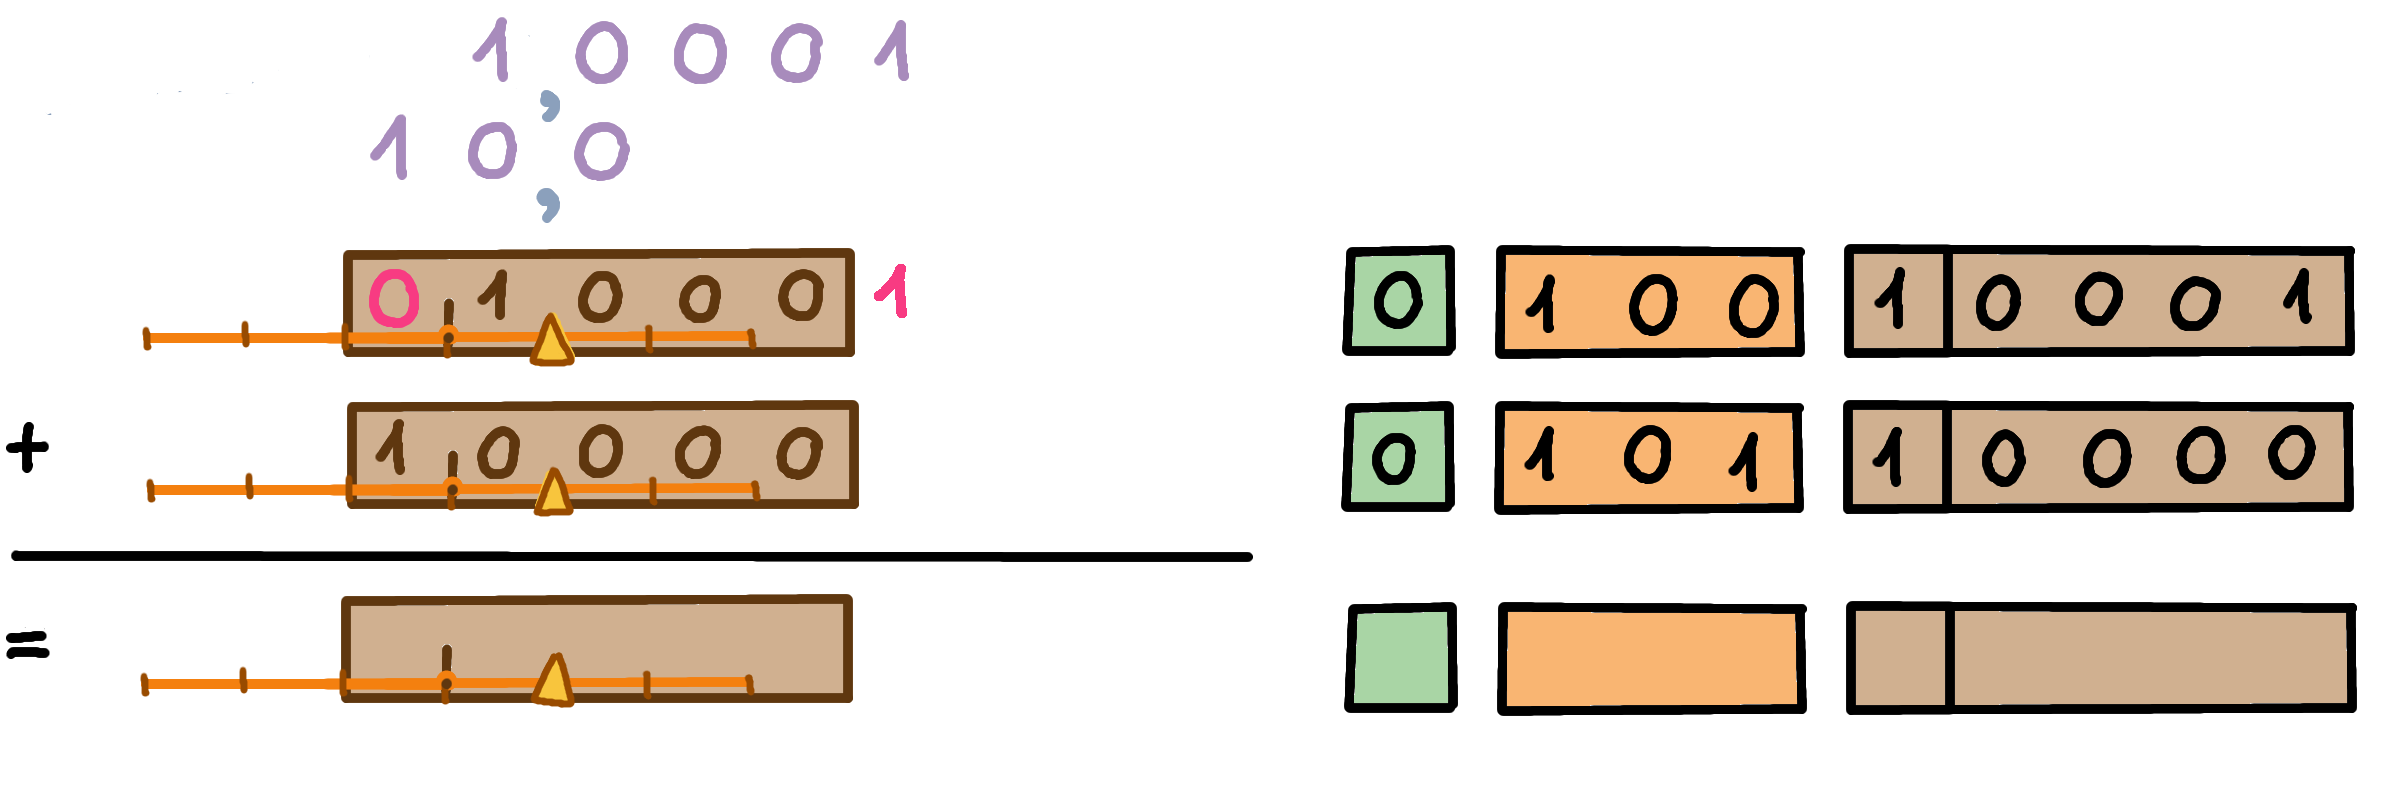
\includegraphics[width=\linewidth]{Pictures/Addition17-16and2_2.png}
\end{figure}

Nun können wir die Bits stellenweise zusammenrechnen.
\begin{figure}[H]
\centering
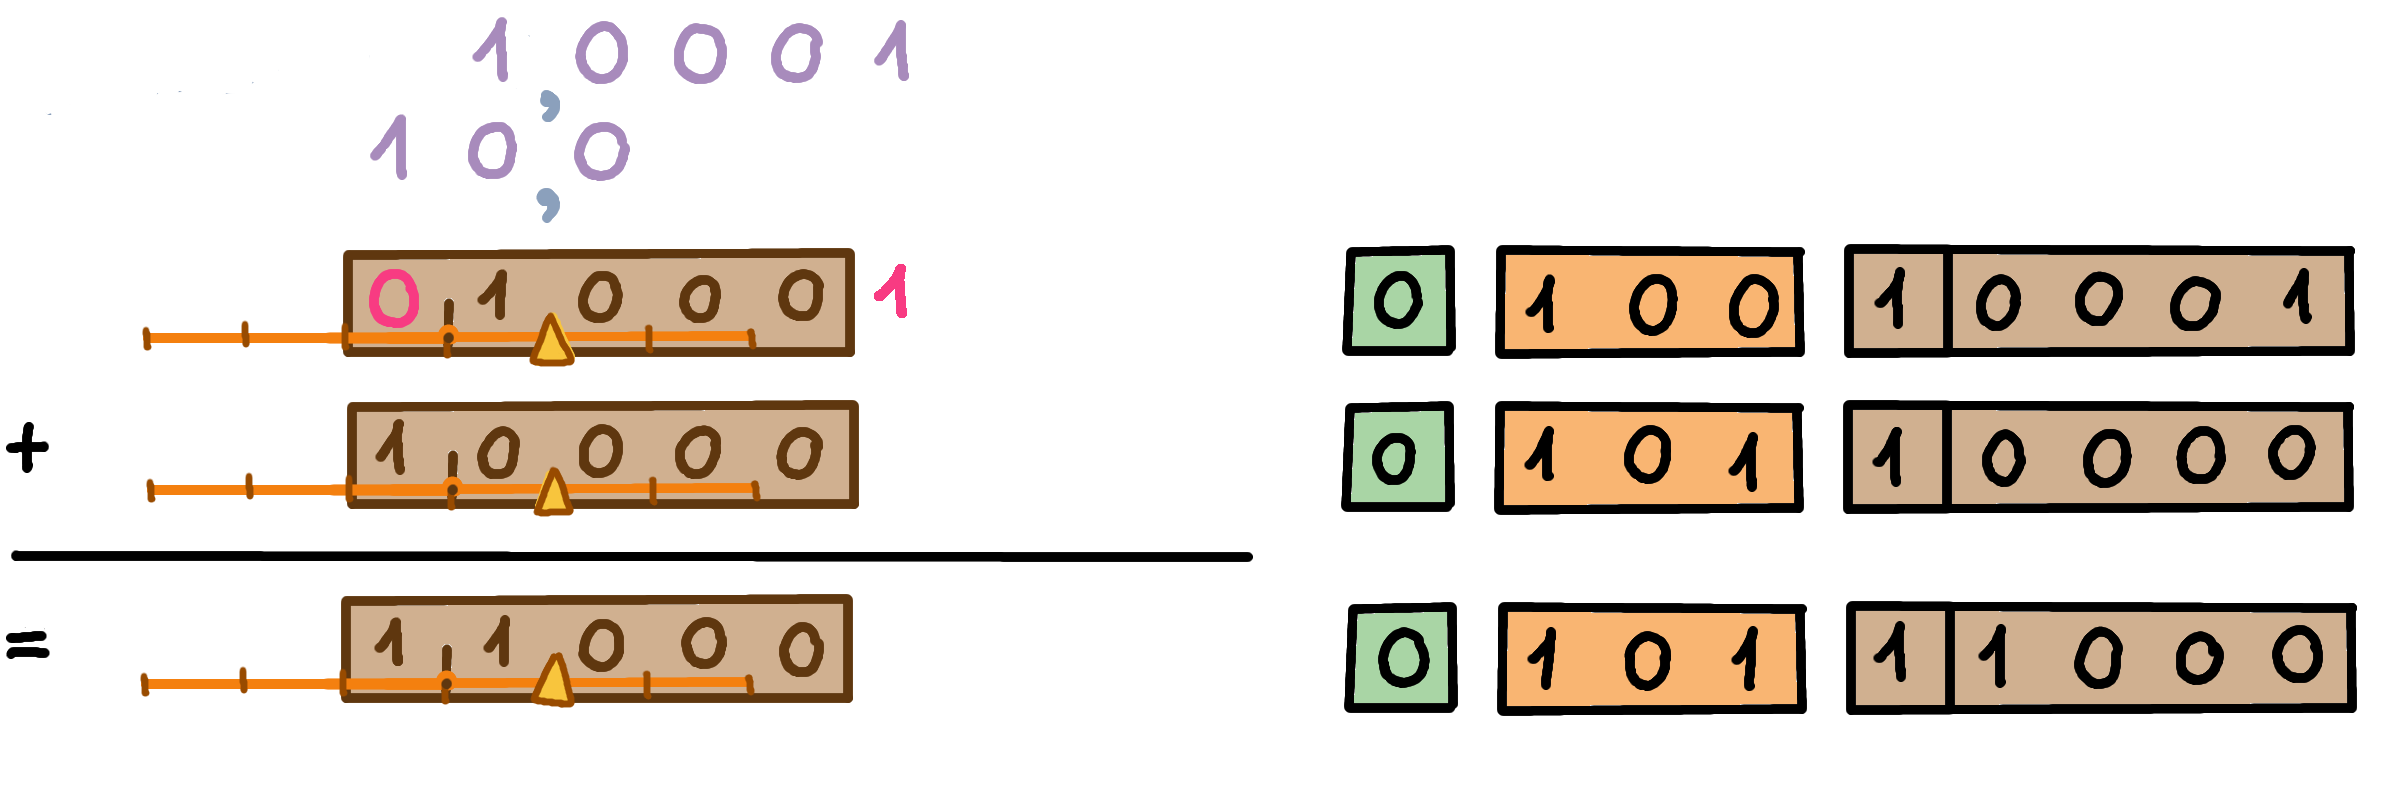
\includegraphics[width=\linewidth]{Pictures/Addition17-16and2_3.png}
\end{figure}

\end{enumerate}

%--------------------------------

\paragraph{Aufgabe \ref{ein_achtel}} Die maximale Zahl, die wir erreichen können, wenn wir \(1/8 + 1/8 + \dotsb + 1/8\) zusammen rechnen, ist \(4.0\).

Zum einen, wenn wir die \(4.0\) erreicht haben, kommen wir nicht mehr weiter.
Das sehen wir, wenn wir \(4.0 + 1/8\) ausrechnen. Wie gewöhnlich schreiben wir zuerst die Summanden untereinander.
\begin{figure}[H]
\centering
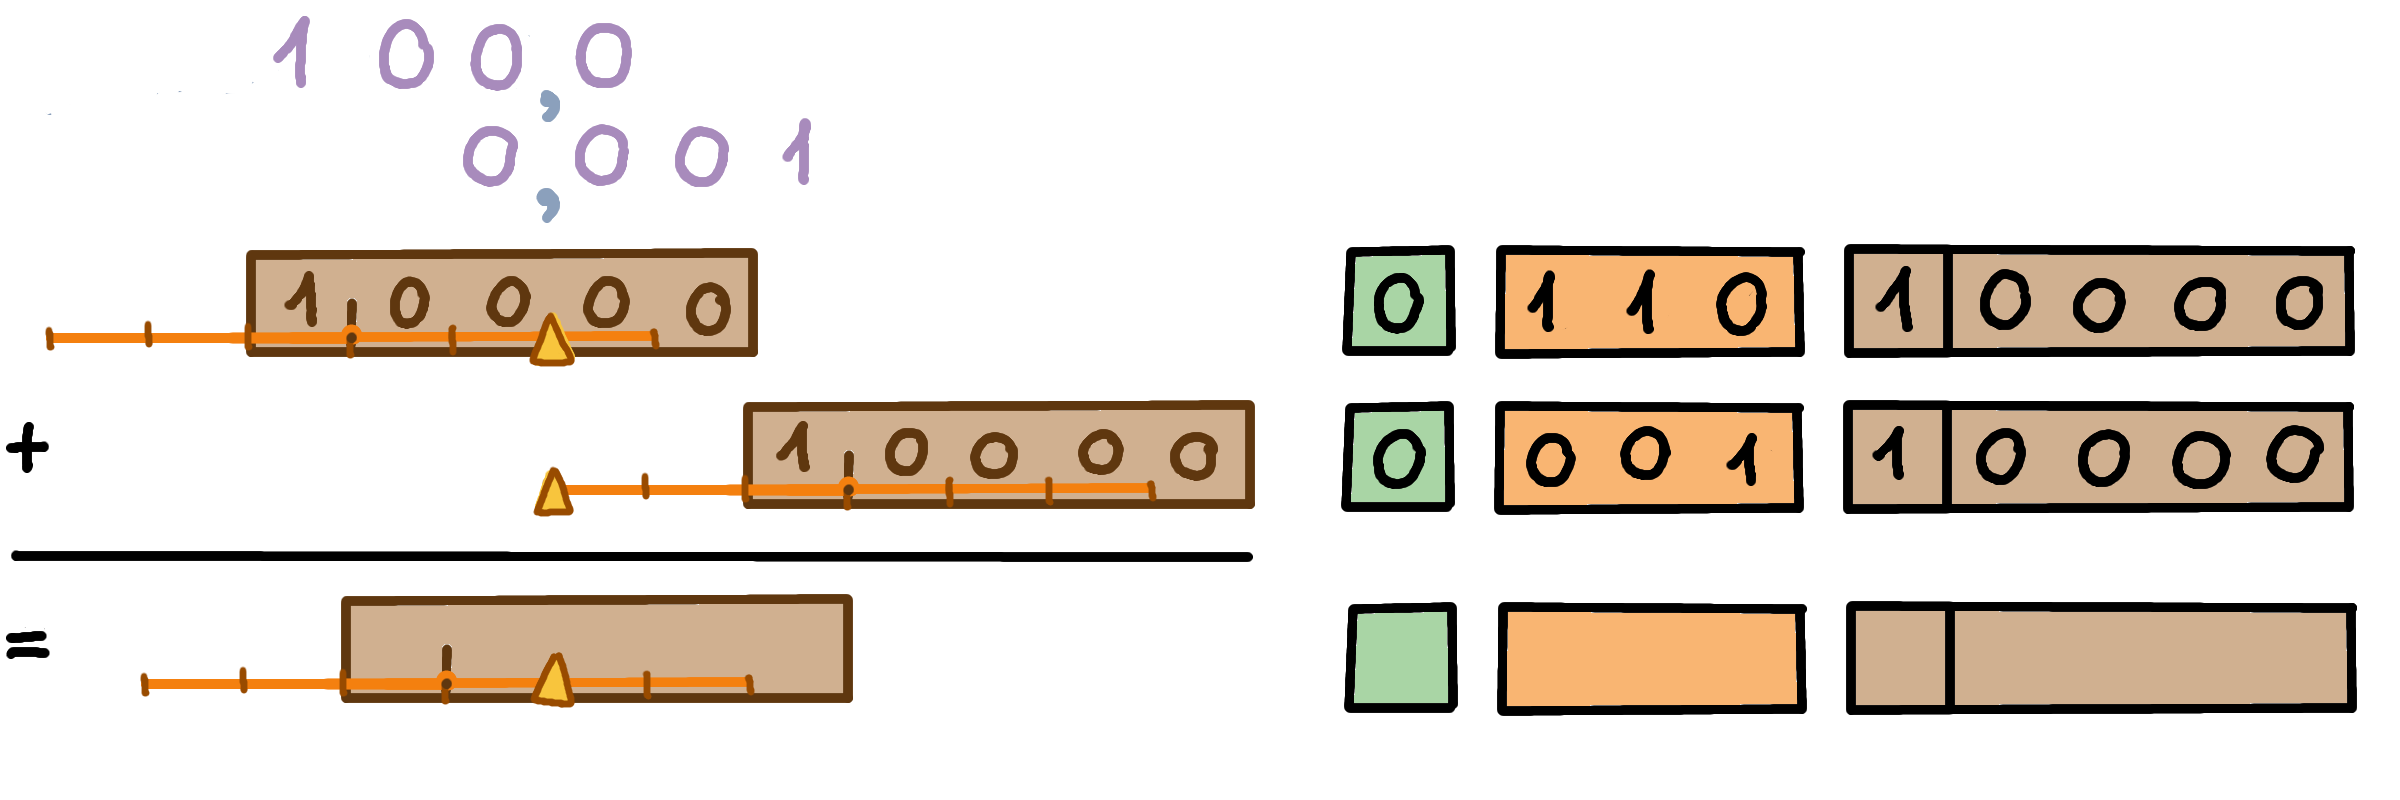
\includegraphics[width=\linewidth]{Pictures/Addition4and1-8_1.png}
\end{figure}
Wenn wir den Kasten von \(1/8\) unter den Kasten von \(4.0\) verschieben, sehen wir, dass alle signifikanten Stellen von \(1/8\) verloren gehen, auch die führende Eins.
\begin{figure}[H]
\centering
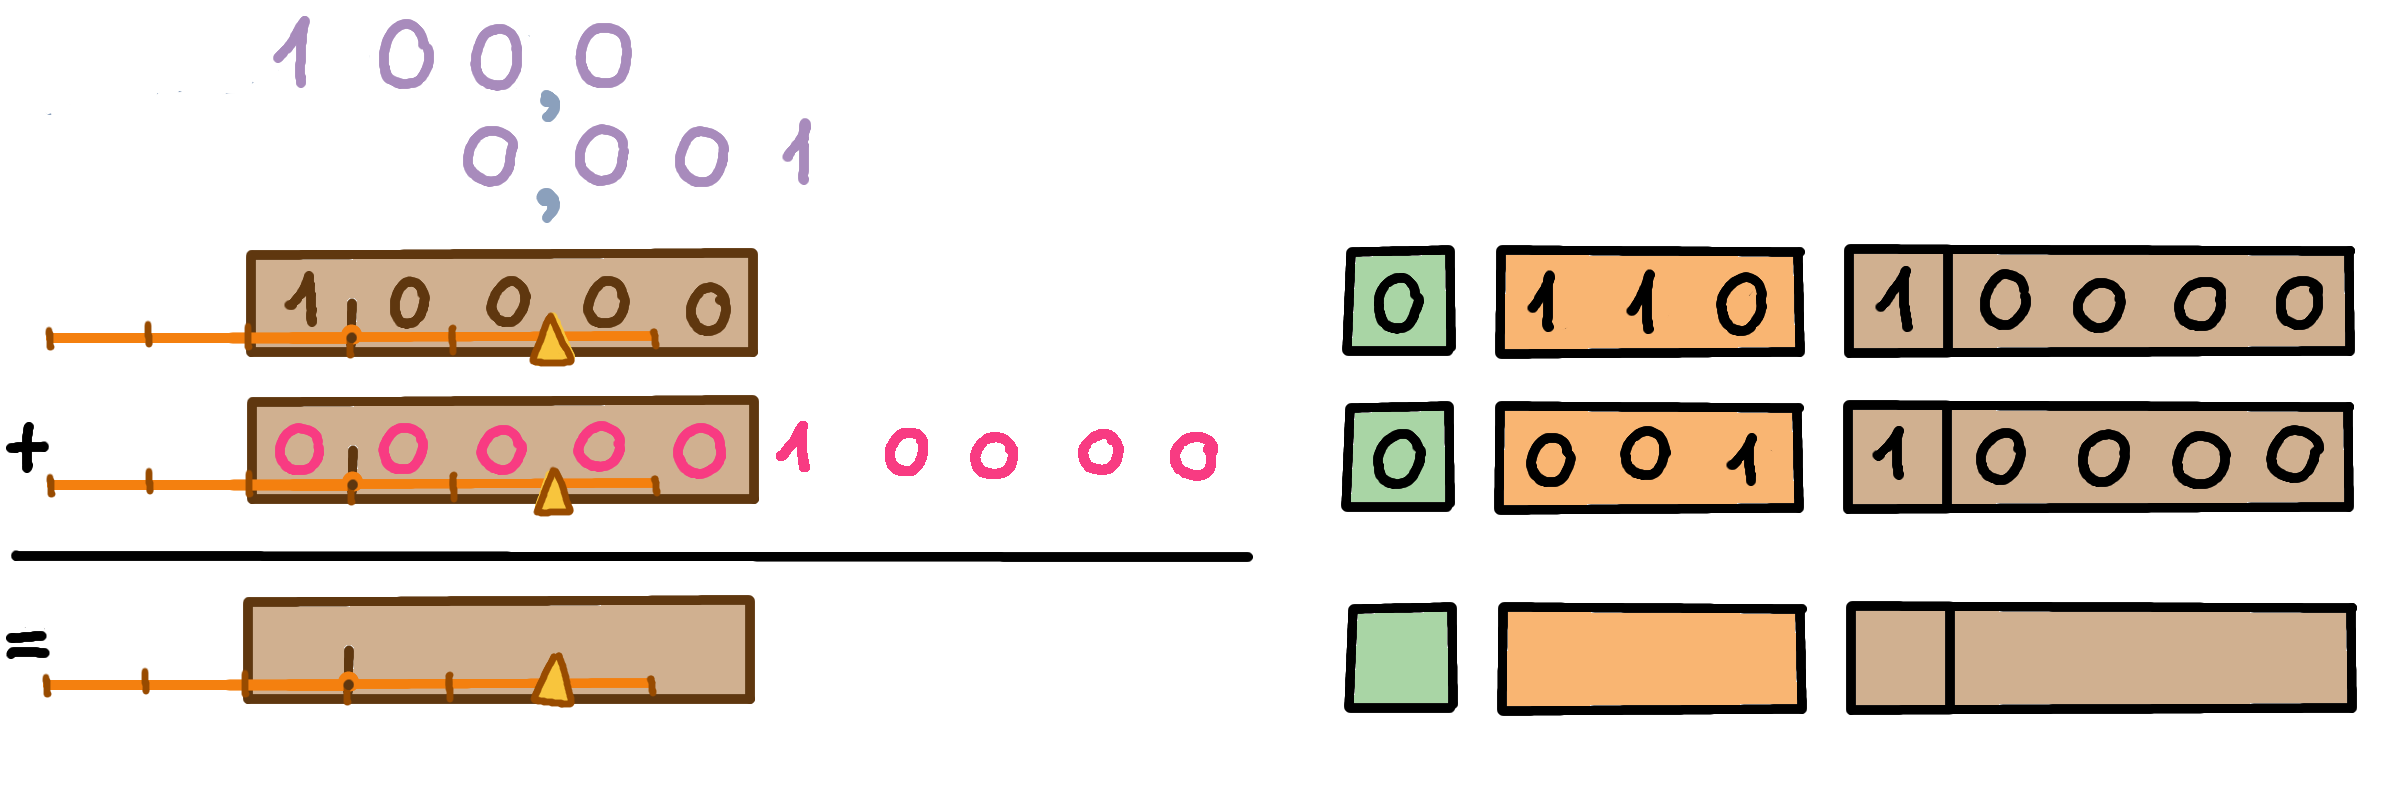
\includegraphics[width=\linewidth]{Pictures/Addition4and1-8_2.png}
\end{figure}
Deswegen, wenn wir \(4.0 + 1/8\) ausrechnen, kriegen wir \(4.0\).
\begin{figure}[H] 
\centering
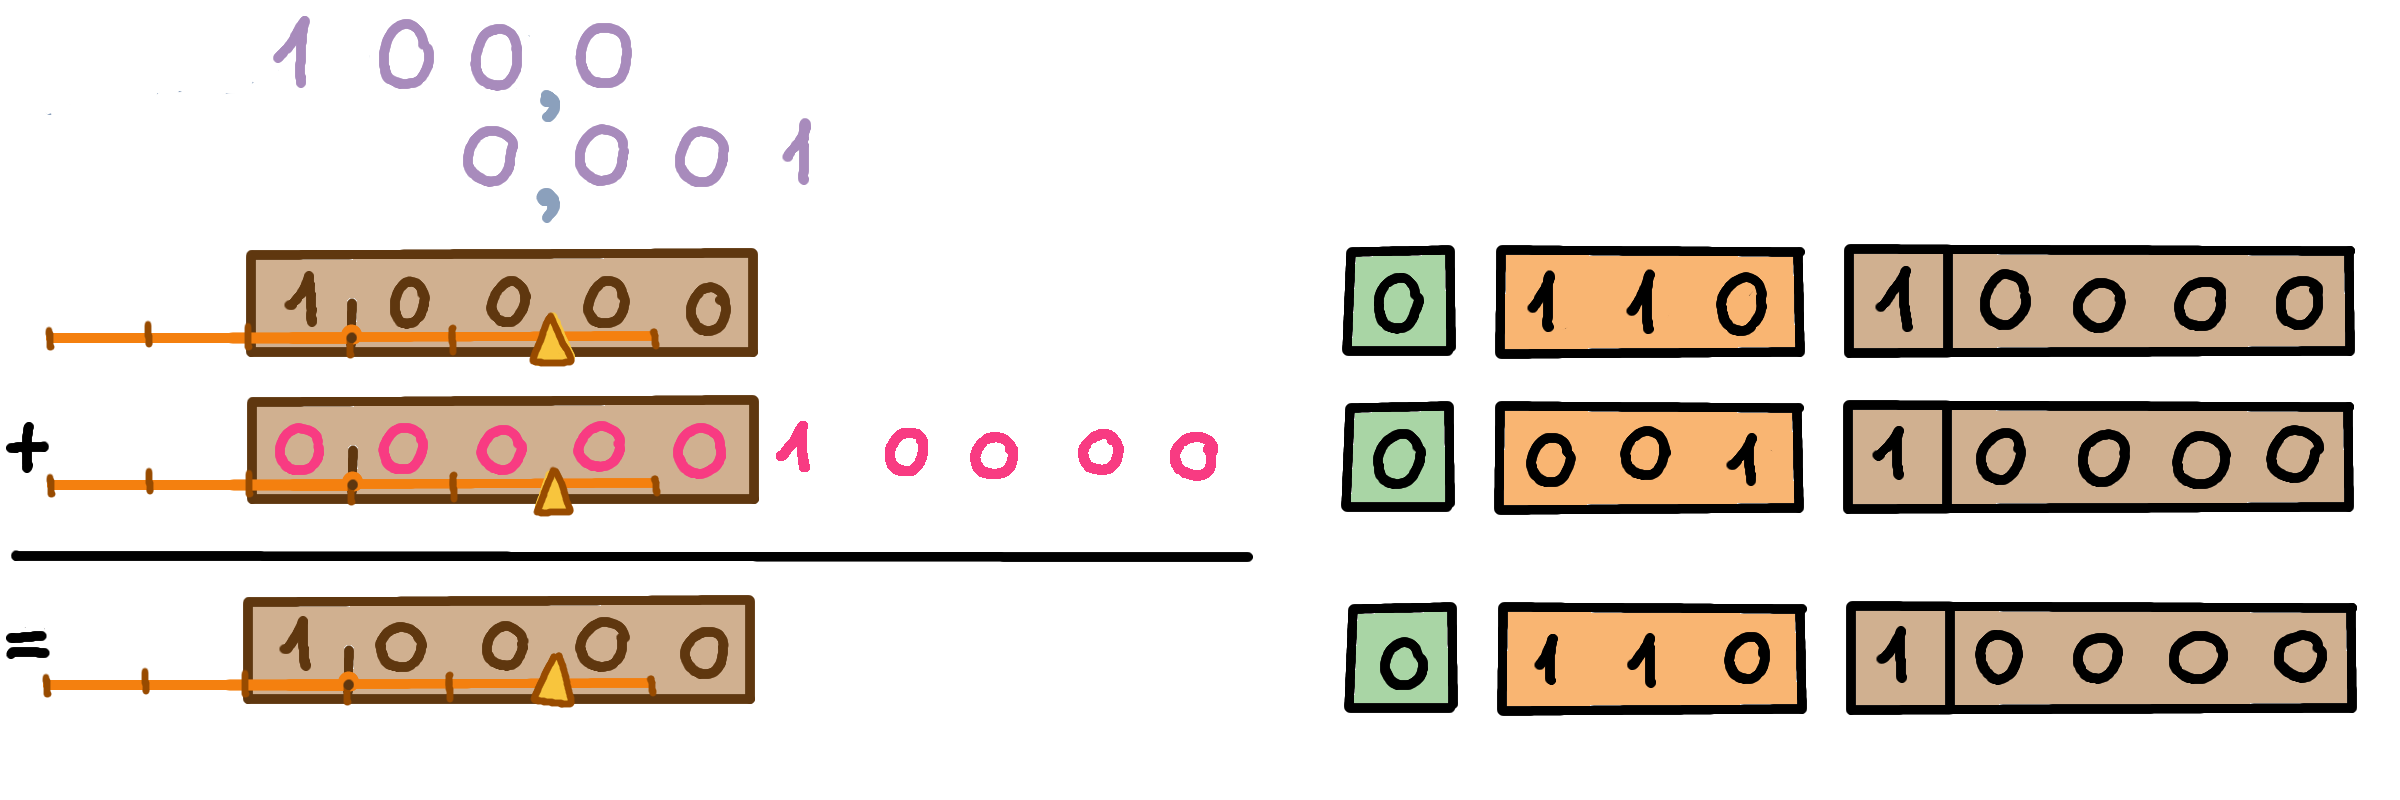
\includegraphics[width=\linewidth]{Pictures/Addition4and1-8_3.png} 
\end{figure}
Egal wie viele \(1/8\) rechnen wir zusammen, bleiben wir immer bei \(4.0\).

Jetzt bleibt uns zu zeigen, dass wir die \(4.0\) auch tatsächlich erreichen können. Das Problem bei der \(4.0\) ist, dass alle signifikanten Stellen von \(1/8\) verloren gehen. Das passiert, weil der Unterschied zwischen dem Exponenten von \(4.0\) und dem Exponenten von \(1/8\) die ganze Mantissenlänge beträgt. Das passiert bei einem kleineren Exponenten nicht. Zum Beispiel, wenn wir \(2.0 + 1/8\) ausrechnen, sehen wir, dass das Ergebnis wie erwartet \(17/8\) ist.

Um zu zeigen, dass das Problem erst bei \(4.0 + 1/8\) auftritt, rechnen wir \(2.0 + 1/8\). Das Ergebnis ist wie erwartet \(17/8\).
\begin{figure}[H]
\centering
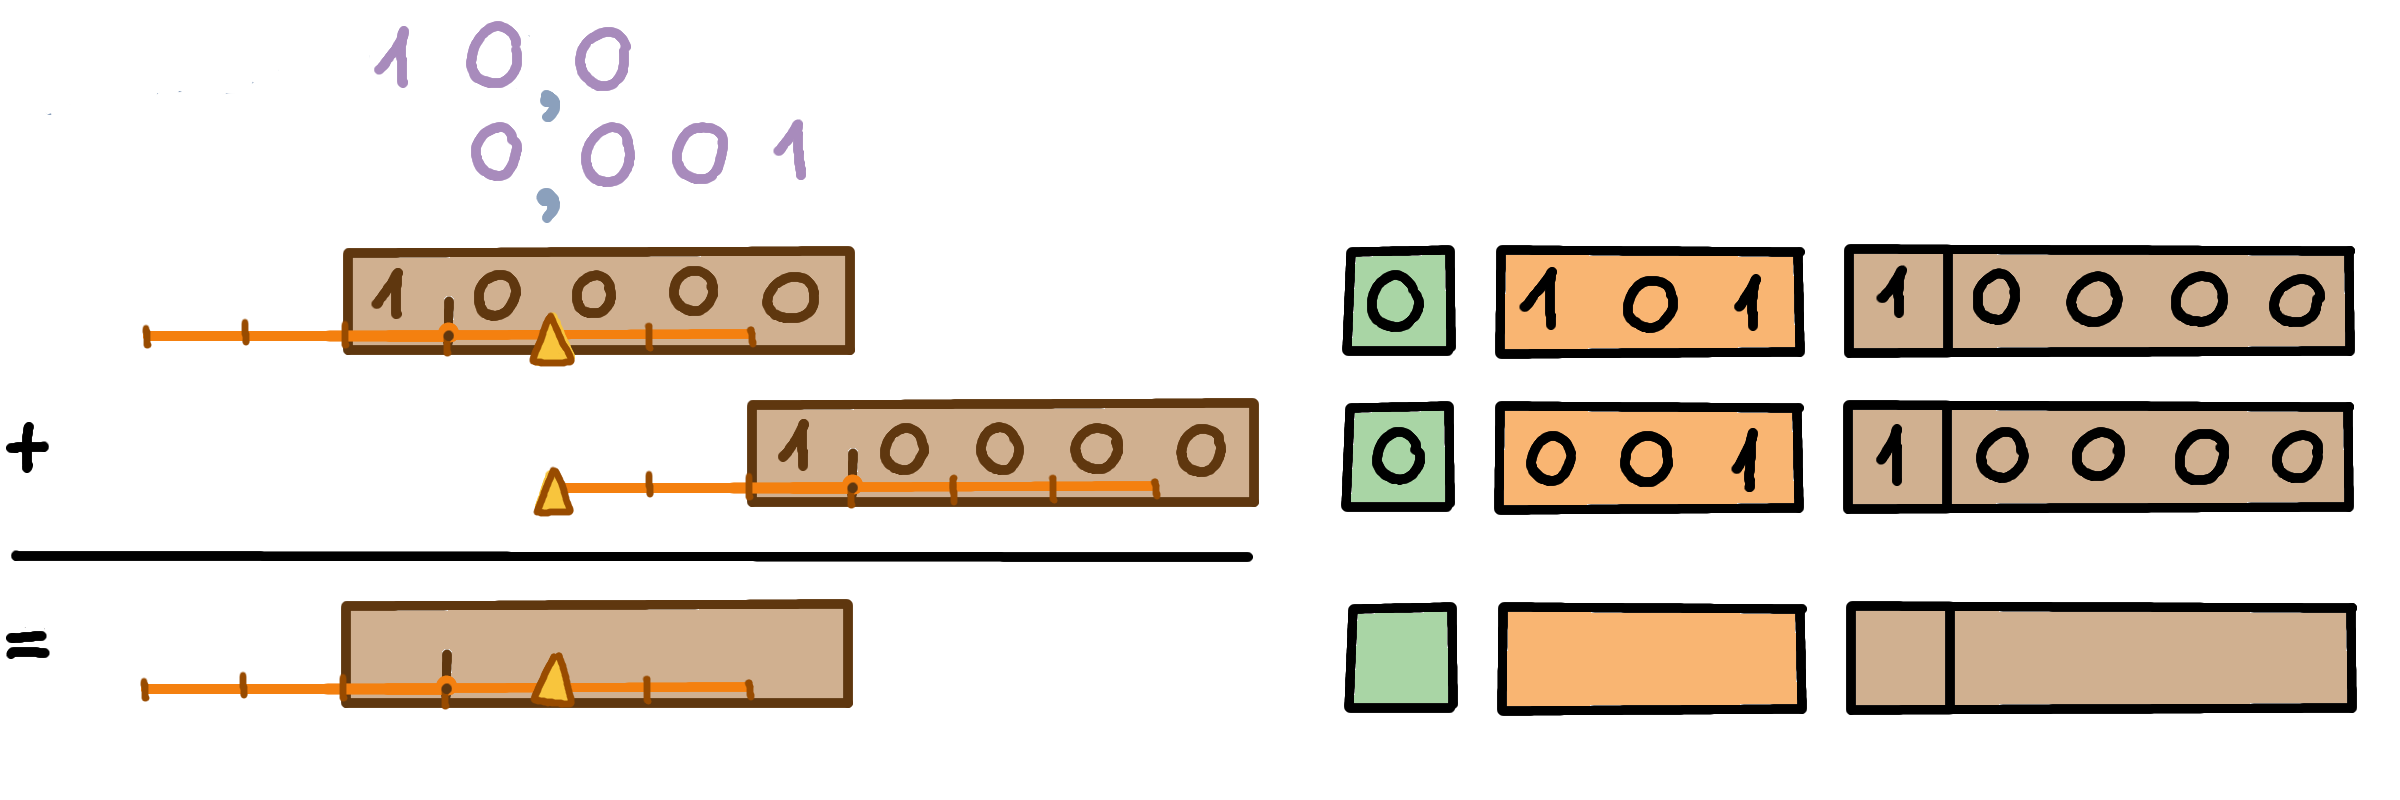
\includegraphics[width=\linewidth]{Pictures/Addition2and1-8_1.png} 
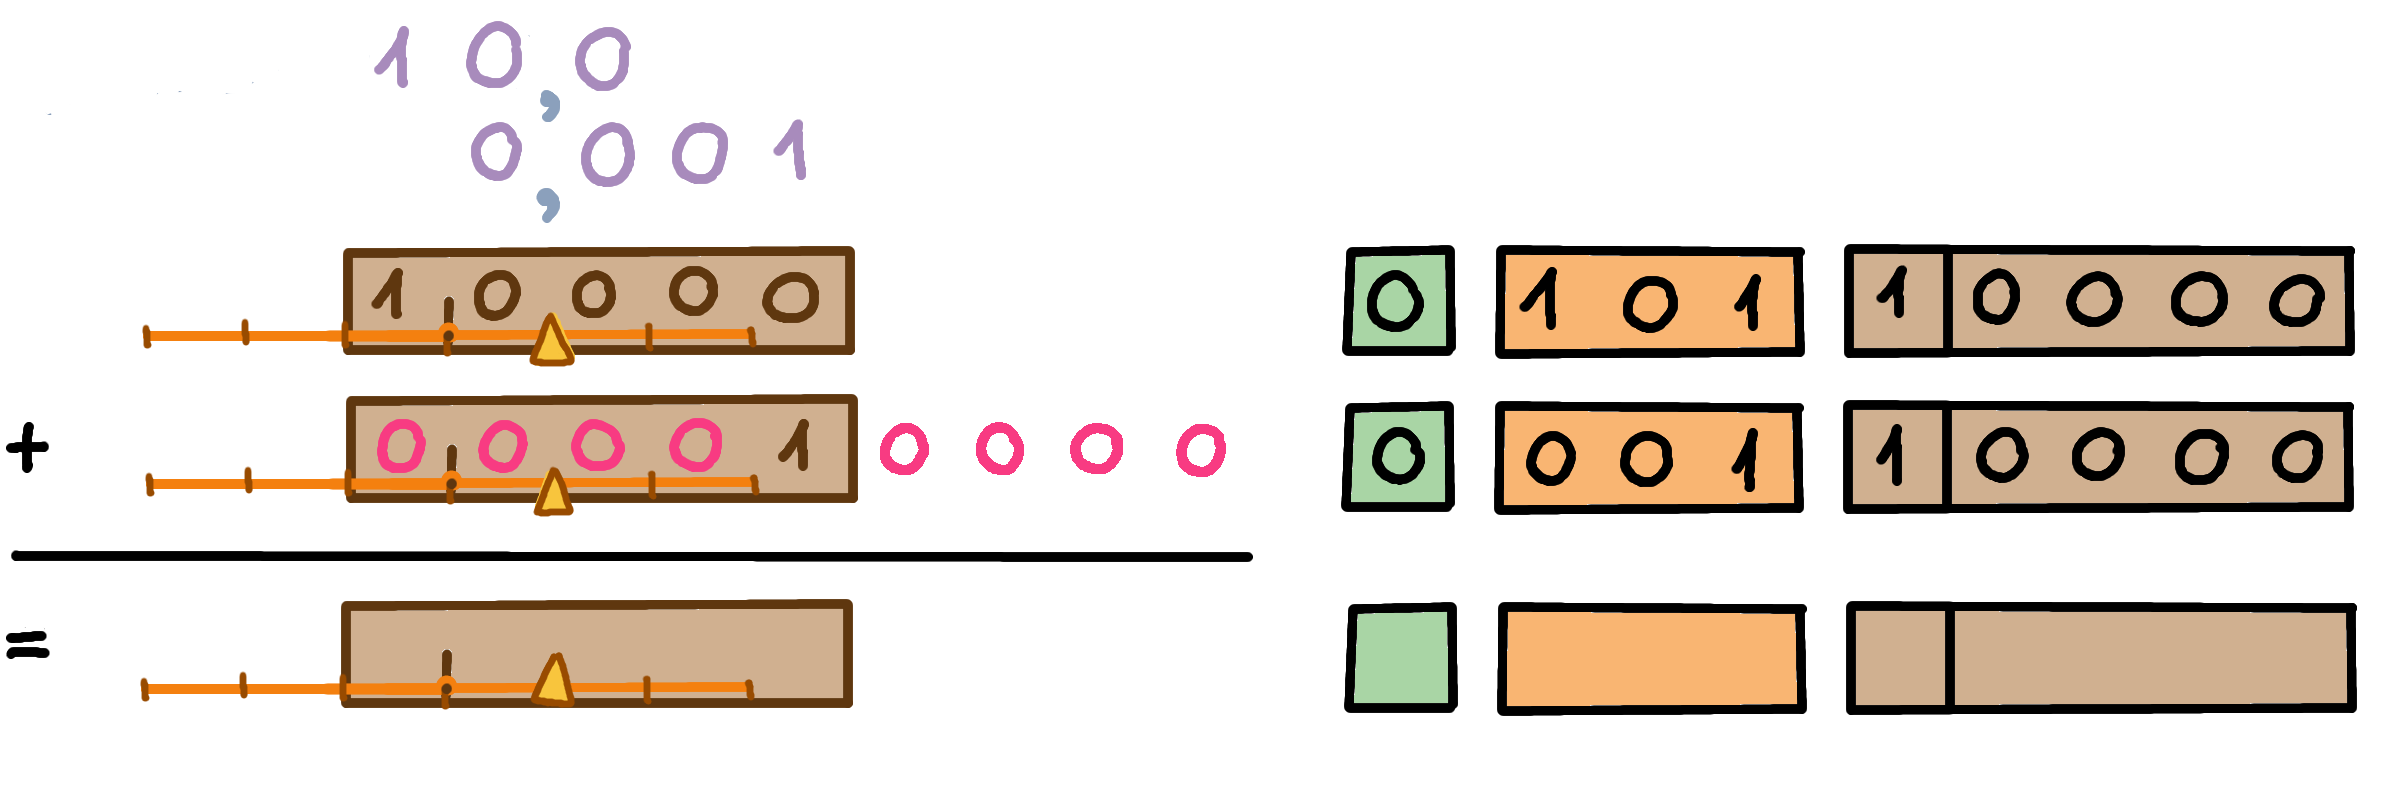
\includegraphics[width=\linewidth]{Pictures/Addition2and1-8_2.png} 
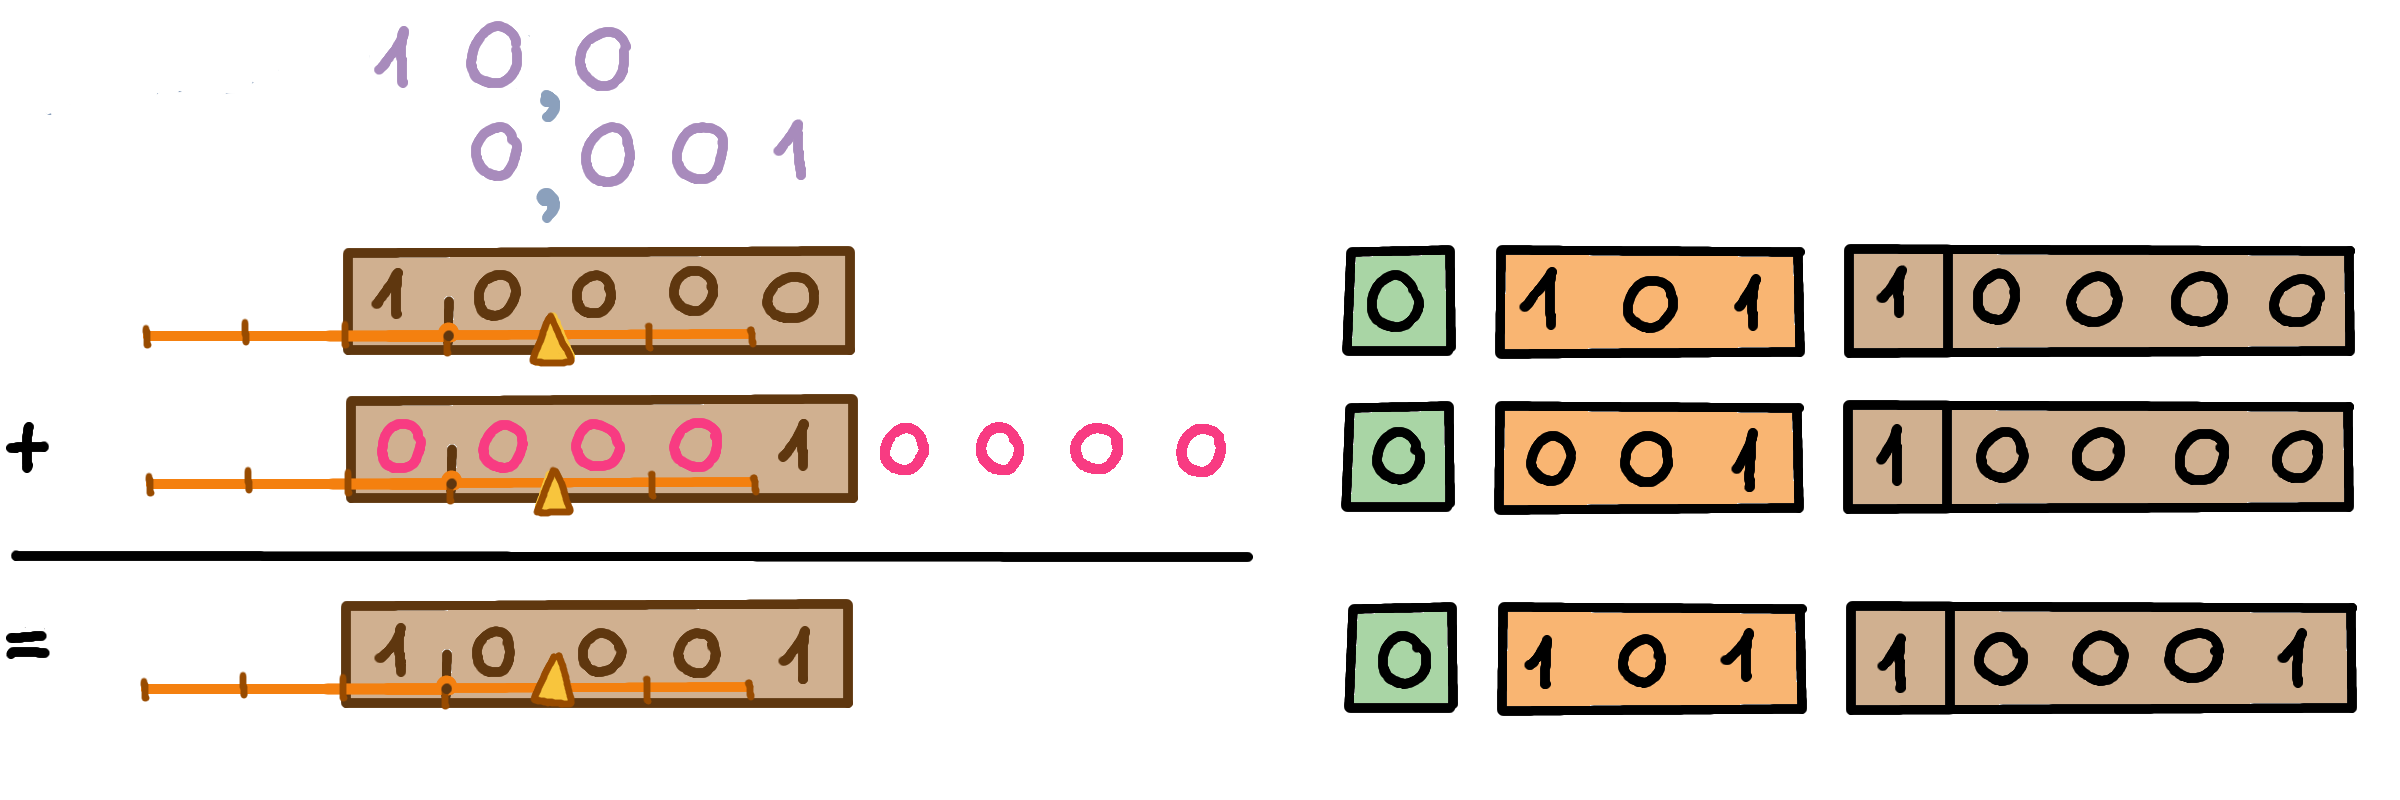
\includegraphics[width=\linewidth]{Pictures/Addition2and1-8_3.png} 
\end{figure}
Wir erreichen also die \(4.0\) nach 32 Summanden und kommen dann nicht mehr weiter.

%--------------------------------

\paragraph{Aufgabe \ref{addition_kontrollfragen}}
\begin{enumerate}[(a)]
\item Der Wert der Bits in der Mantisse hängt vom Exponenten ab. Zum Beispiel, dieselbe Mantisse \(1.0000\) mit unterschiedlichen Exponenten kann \(4\), \(2\), \(1\), \(1/2\), \(1/4\) und \(1/8\) darstellen. Wir wollen nicht, dass \(1+2\) das gleiche Ergebnis liefert die \(1 + 1/4\). Wir wollen nur Bits mit dem gleichen Wert zusammen addieren. Deswegen müssen wir vor der Addition sicherstellen, dass die Kasten der beiden Summanden exakt untereinander stehen.

\item Die Aussage von Gregory ist falsch. Der Kasten vom Ergebnis kann sich bewegen bezüglich des Kastens vom grössten Summanden. Dies passiert, zum Beispiel, wenn man \(2.5 + 1.75\) ausrechnet.

\item Hannah hat teilweise recht. Die Addition bei den Fliesskommazahlen ist kommutativ aber nicht assoziativ.

Wenn wir zwei Zahlen zusammen addieren und diese zwei Zahlen vertauschen, kriegen wir das gleiche Ergebnis auch bei Fliesskommazahlen.

Wenn wir aber die Reihenfolge verändern, in welcher die Zahlen zusammengerechnet werden, können wir unterschiedlich Ergebnisse bekommen. Das passiert, weil wir nur dann den exakten Wert ausrechnen können, wenn die Grössenordnung der Teilsummanden ähnlich ist.
\end{enumerate}

%--------------------------------

\paragraph{Aufgabe \ref{ameisenkönigin}}

Nein, das Programm der Ameisenkönigin wird unendlich lange laufen und die Anzahl Ameisen, die es braucht, um 10 Reiskörnchen zu transportieren, nie ausgeben. Das Problem ist analog zu dem, was wir in Aufgabe \ref{ein_achtel} gesehen haben. Das Programm läuft wie erwartet bis wir die \(8.0\) erreichen. Wenn wir aber \(1/4\) dazu rechnen, dann verlieren wir alle signifikanten Stellen von \(1/4\) und die \(8.0\) bleibt unverändert.
\begin{figure}[H]
\centering
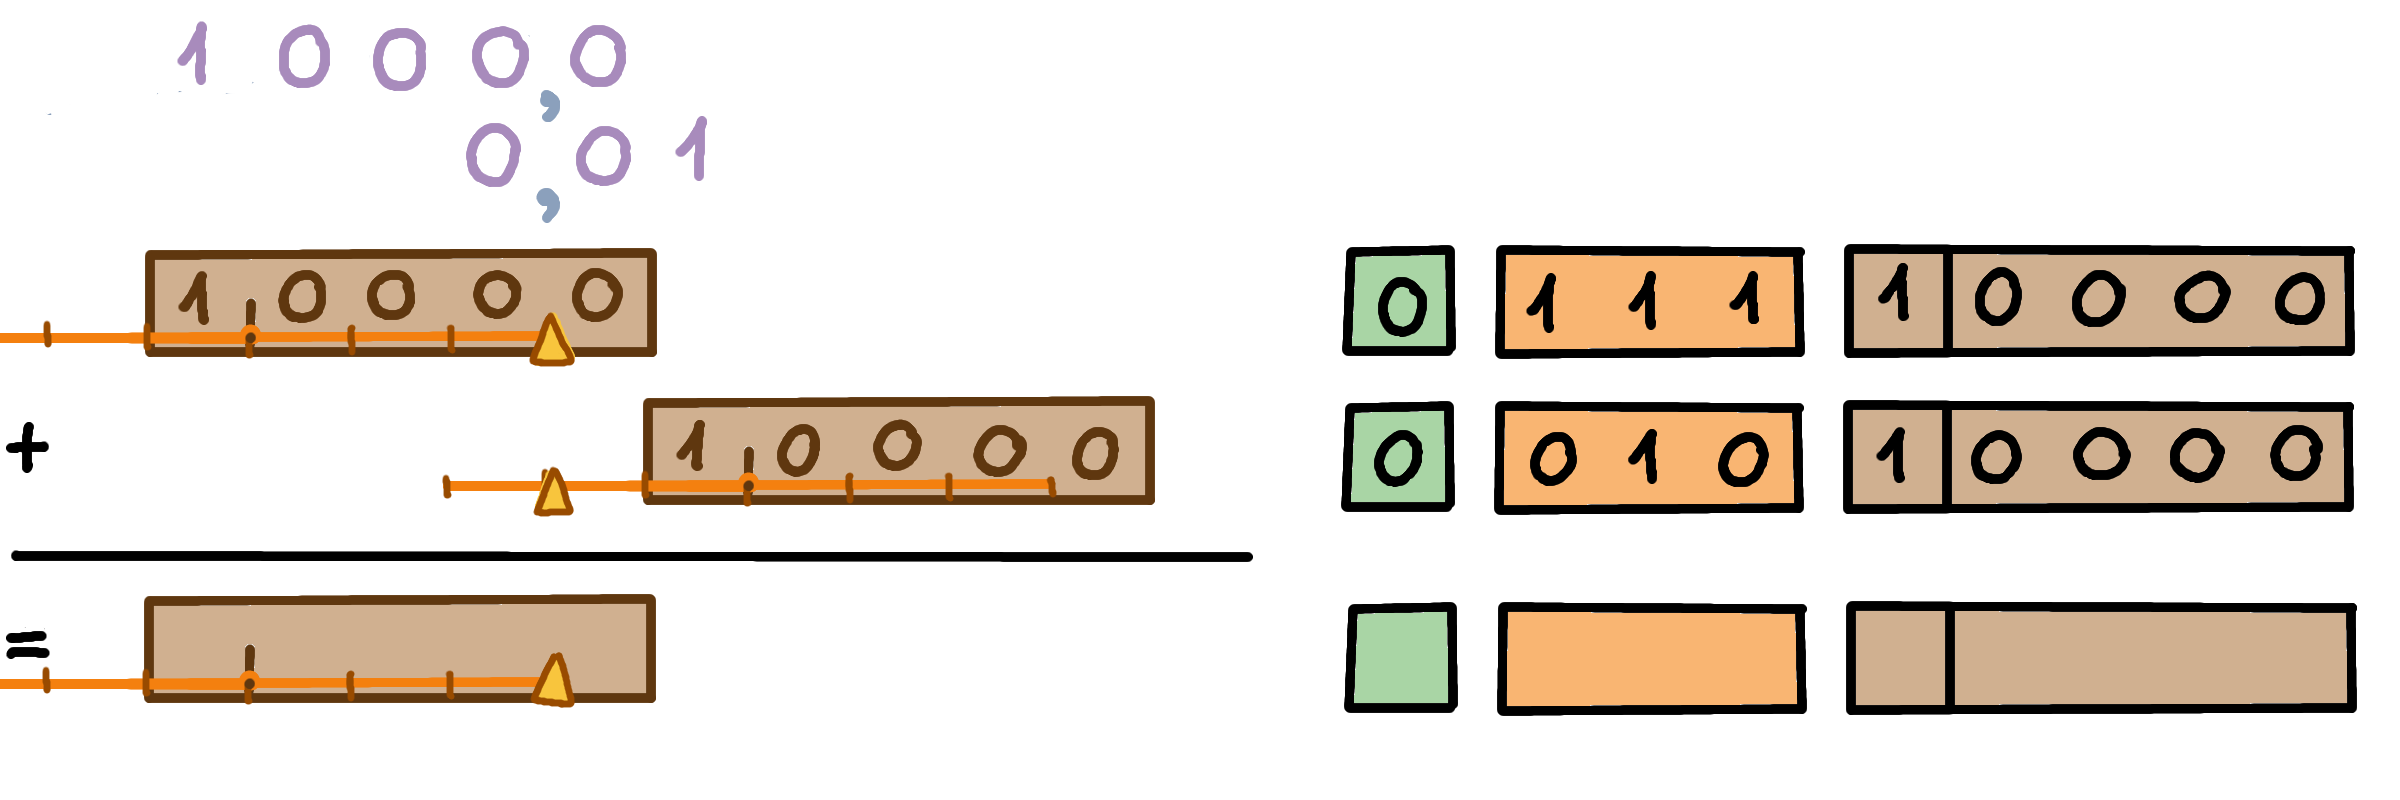
\includegraphics[width=\linewidth]{Pictures/Addition8and1-4_1.png} 
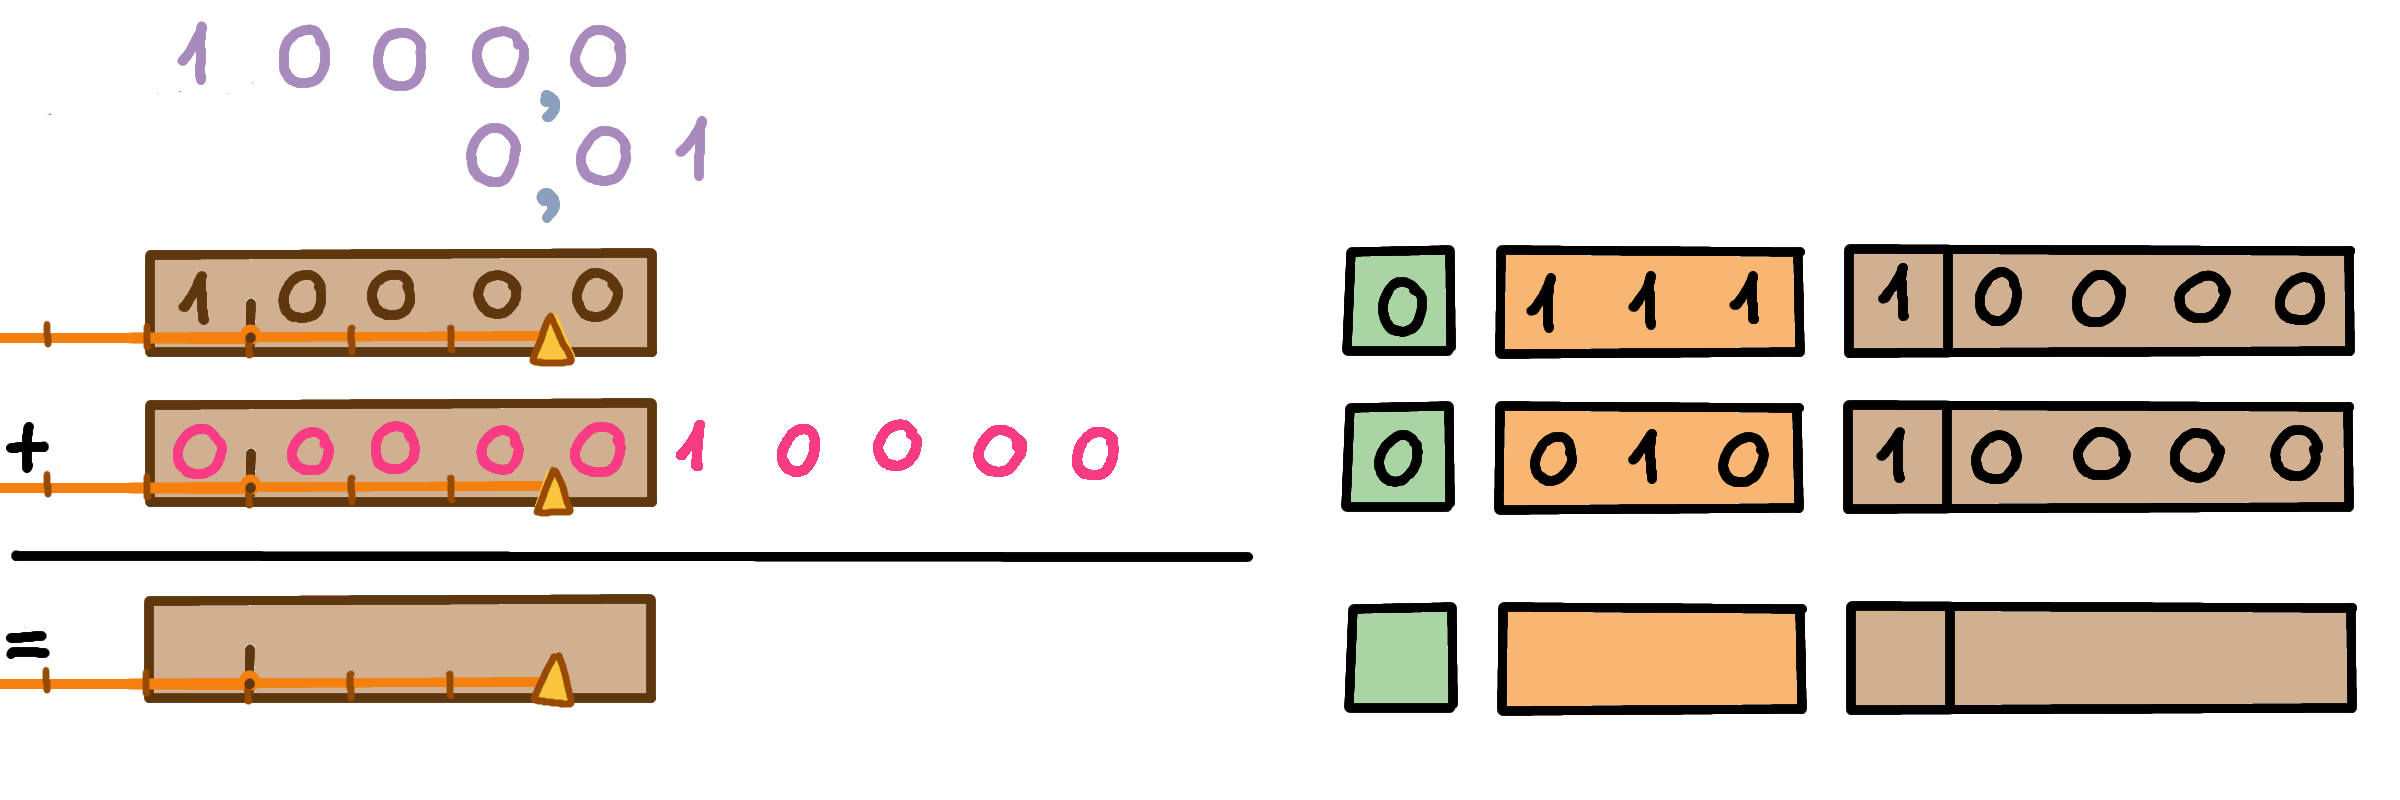
\includegraphics[width=\linewidth]{Pictures/Addition8and1-4_2.png} 
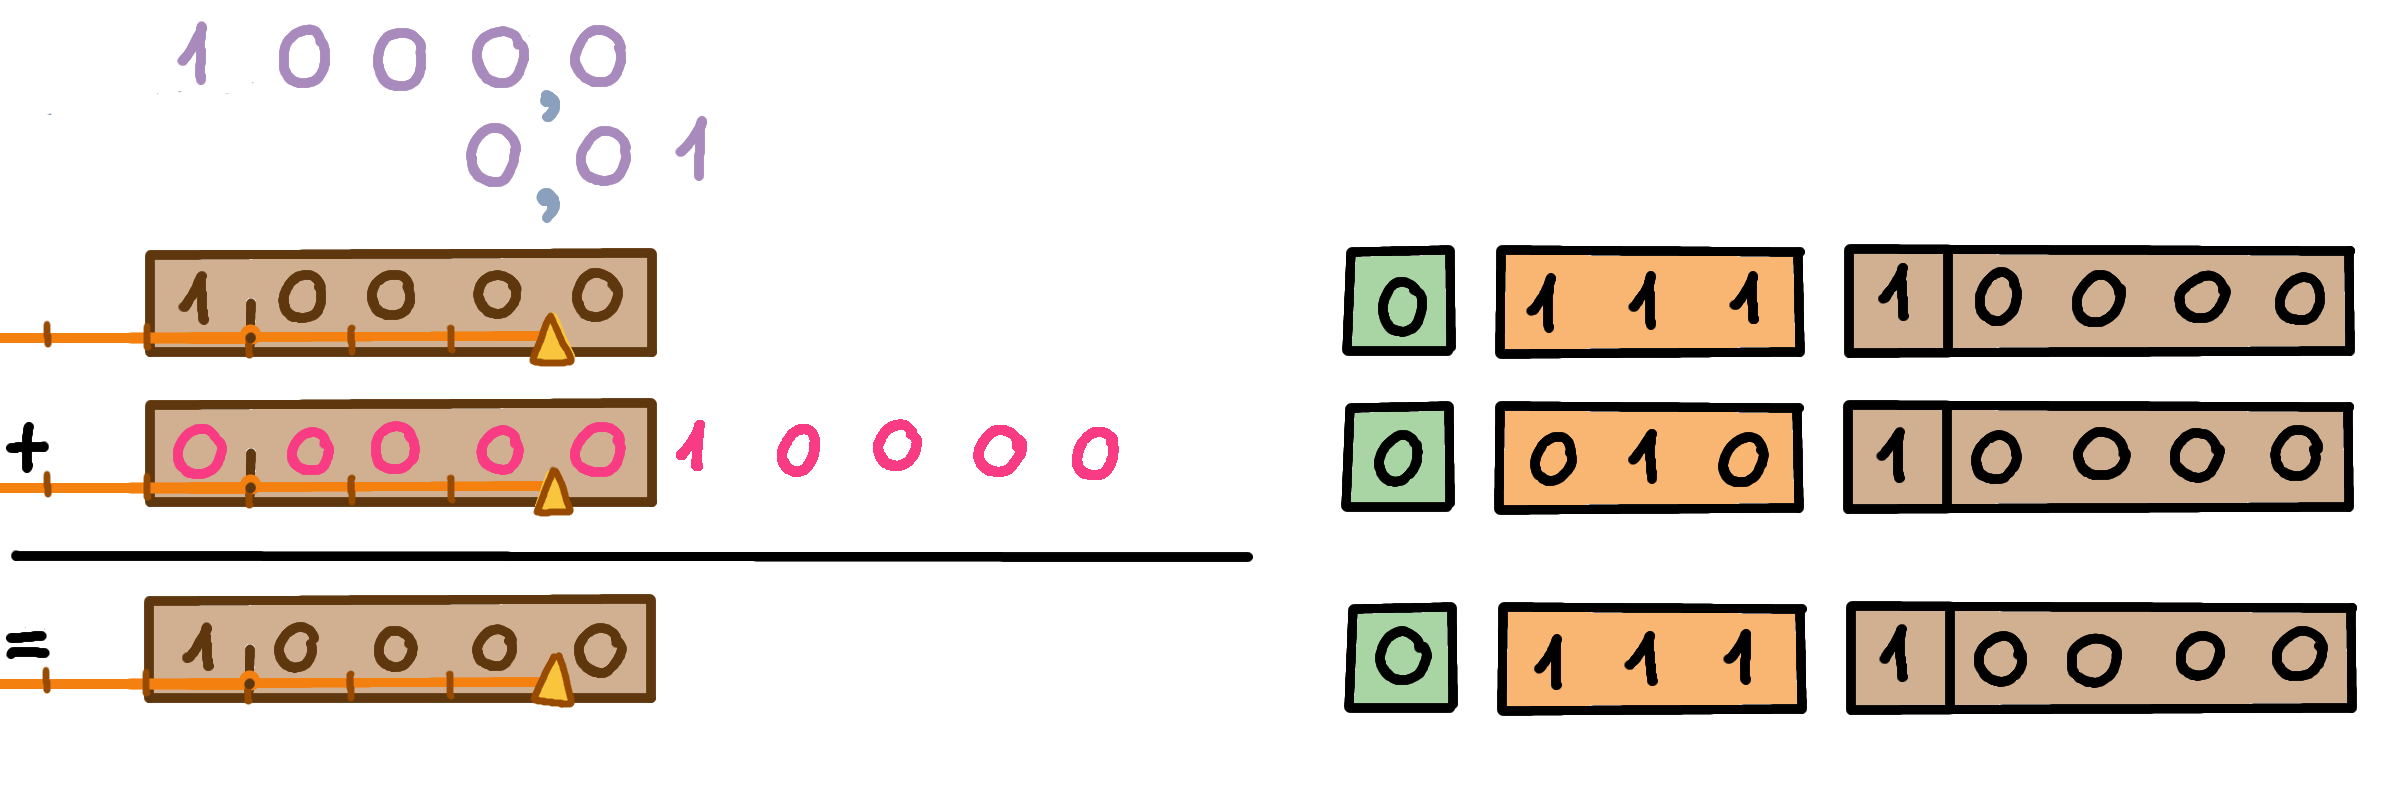
\includegraphics[width=\linewidth]{Pictures/Addition8and1-4_3.png} 
\end{figure}